\documentclass[12pt]{article}\usepackage[]{graphicx}\usepackage[]{color}
%% maxwidth is the original width if it is less than linewidth
%% otherwise use linewidth (to make sure the graphics do not exceed the margin)
\makeatletter
\def\maxwidth{ %
  \ifdim\Gin@nat@width>\linewidth
    \linewidth
  \else
    \Gin@nat@width
  \fi
}
\makeatother

\definecolor{fgcolor}{rgb}{0.345, 0.345, 0.345}
\newcommand{\hlnum}[1]{\textcolor[rgb]{0.686,0.059,0.569}{#1}}%
\newcommand{\hlstr}[1]{\textcolor[rgb]{0.192,0.494,0.8}{#1}}%
\newcommand{\hlcom}[1]{\textcolor[rgb]{0.678,0.584,0.686}{\textit{#1}}}%
\newcommand{\hlopt}[1]{\textcolor[rgb]{0,0,0}{#1}}%
\newcommand{\hlstd}[1]{\textcolor[rgb]{0.345,0.345,0.345}{#1}}%
\newcommand{\hlkwa}[1]{\textcolor[rgb]{0.161,0.373,0.58}{\textbf{#1}}}%
\newcommand{\hlkwb}[1]{\textcolor[rgb]{0.69,0.353,0.396}{#1}}%
\newcommand{\hlkwc}[1]{\textcolor[rgb]{0.333,0.667,0.333}{#1}}%
\newcommand{\hlkwd}[1]{\textcolor[rgb]{0.737,0.353,0.396}{\textbf{#1}}}%

\usepackage{framed}
\makeatletter
\newenvironment{kframe}{%
 \def\at@end@of@kframe{}%
 \ifinner\ifhmode%
  \def\at@end@of@kframe{\end{minipage}}%
  \begin{minipage}{\columnwidth}%
 \fi\fi%
 \def\FrameCommand##1{\hskip\@totalleftmargin \hskip-\fboxsep
 \colorbox{shadecolor}{##1}\hskip-\fboxsep
     % There is no \\@totalrightmargin, so:
     \hskip-\linewidth \hskip-\@totalleftmargin \hskip\columnwidth}%
 \MakeFramed {\advance\hsize-\width
   \@totalleftmargin\z@ \linewidth\hsize
   \@setminipage}}%
 {\par\unskip\endMakeFramed%
 \at@end@of@kframe}
\makeatother

\definecolor{shadecolor}{rgb}{.97, .97, .97}
\definecolor{messagecolor}{rgb}{0, 0, 0}
\definecolor{warningcolor}{rgb}{1, 0, 1}
\definecolor{errorcolor}{rgb}{1, 0, 0}
\newenvironment{knitrout}{}{} % an empty environment to be redefined in TeX

\usepackage{alltt}

\usepackage{amssymb,amsmath}
\usepackage{enumerate}
\usepackage{float}
\usepackage{verbatim}
\usepackage{setspace}
\usepackage{multicol}

%% LaTeX margin settings:
  \setlength{\textwidth}{7.0in}
\setlength{\textheight}{9in}
\setlength{\oddsidemargin}{-.5in}
\setlength{\evensidemargin}{0in}
\setlength{\topmargin}{-1.5cm}

%% tell knitr to use smaller font for code chunks
\def\fs{\footnotesize}
\def\R{{\sf R}}
\newcommand{\bfbeta}{\mbox{\boldmath $\beta$}}
\newcommand{\bfD}{\mbox{\boldmath $D$}}
\newcommand{\bfL}{\mbox{\boldmath $L$}}
\newcommand{\bfR}{\mbox{\boldmath $R$}}
\newcommand{\bfmu}{\mbox{\boldmath $\mu$}}
\newcommand{\bfv}{\mbox{\boldmath $V$}}
\newcommand{\bfX}{\mbox{\boldmath $X$}}
\newcommand{\bfy}{\mbox{\boldmath $y$}}
\newcommand{\bfb}{\mbox{\boldmath $b$}}
\newcommand{\ytil}{\mbox{$\tilde{y}$}}
\IfFileExists{upquote.sty}{\usepackage{upquote}}{}
\begin{document}


  
  
\begin{center}
\large{Bayes: Homework $4$} \\
Leslie Gains-Germain
\end{center}

\begin{doublespacing}

{\bf Problem 1}

\begin{enumerate}

\item I chose a $Gam(20, 1)$ prior for $\lambda$, and the sum of the $x$'s was $409$ in the fake date that I generated. The posterior distribution of $\lambda|x$ is then $Gam(429, 21)$. The code is included in the appendix, and the quantities of interest are shown in the following table for different sample sizes.

\begin{table} [h!]
\centering
\begin{tabular} {c|c|c|c}
Sample Size & $90\%$ posterior interval & $Pr(10 < x < 20)$ & $Pr(x < 5)$ \\
\hline 
10 & (19.51, 20.88) & 0.50 & 0 \\
50 & (19.02, 22.80) & 0.26 & 0 \\
100 & (18.57, 22.01) & 0.31 & 0 \\
250 & (18.90, 22.13) & 0.30 & 0 \\
1000 & (18.78, 22.03) & 0.36 & 0 \\
10000 & (18.81, 22.08) & 0.34 & 0 \\
Theoretical Distribution & (18.84, 22.08) & 0.34 & $\approx 0$ \\
\hline
\end{tabular}
\end{table}

The posterior interval and posterior probabilities get closer to the theoretical quantities as the sample size increases. At a sample size of $10$, the posterior interval and probabilities can change dramatically if you get one unusual draw. For sample sizes less than $1000$, the quantities also can change depending on the draws obtained. For example, the posterior interval at a sample size of $50$ is wider than $10$ because I obtained draws in the tails of the distribution. At a sample size of $10$, only the more probable values in the middle of the distribution are obtained. This could be reversed, however, if I happened to draw an unusual value in the sample of size $10$. At a sample of size $10000$, the quantiles and probabilities are very similar to those from the theoretical distribution. I think the main point is that if you are trying to characterize a posterior distribution by pulling random draws from it, you need a large sample size (10000 or more!) to appropriately characterize the distribution.




\item Below I obtain $1000$ draws from a $Gam(429, 21)$ using the grid approximation method. I used grid sizes of $0.5$, $0.1$, $0.01$, $0.001$ and $0.00001$. It looks like the grid size of $0.5$ gave the worst approximation because values less than $21$ were overrepressented and values greater than $21$ were underrepresented overall. At grid sizes of $0.1$ and $0.01$, the approximation still looks shifted left a little bit with values less than $21$ overrepresented (although not as bad as the $0.5$ case). It looks like the approximation was fairly equivalent at grid sizes of $0.001$ and $0.00001$. In practice, I would use a grid size of $0.001$ because it looks like you get the best compromise between computing power and the quality of the approximation.

\begin{singlespace}
\begin{knitrout}\footnotesize
\definecolor{shadecolor}{rgb}{0.969, 0.969, 0.969}\color{fgcolor}\begin{kframe}
\begin{alltt}
\hlcom{#function to calculate posterior probabilities}
\hlstd{posterior} \hlkwb{<-} \hlkwa{function}\hlstd{(}\hlkwc{x}\hlstd{)\{}
  \hlkwd{dgamma}\hlstd{(x,} \hlnum{429}\hlstd{,} \hlnum{21}\hlstd{)}
\hlstd{\}}

\hlcom{#possible x values}
\hlcom{#use small grid size}
\hlstd{xsmall} \hlkwb{<-} \hlkwd{seq}\hlstd{(}\hlnum{15}\hlstd{,} \hlnum{25}\hlstd{,} \hlnum{.00001}\hlstd{)}

\hlcom{##sample x with probability proportional to height of function within that grid}
\hlkwd{set.seed}\hlstd{(}\hlnum{17}\hlstd{)}
\hlstd{grid.draws} \hlkwb{<-} \hlkwd{sample}\hlstd{(xsmall,} \hlnum{1000}\hlstd{,} \hlkwc{prob}\hlstd{=}\hlkwd{posterior}\hlstd{(xsmall))}

\hlcom{#plot draws with posterior overlaid}
\hlcom{#hist(grid.draws, freq=F, main="grid size 0.00001")}
\hlcom{#lines(xsmall, posterior(xsmall))}
\end{alltt}
\end{kframe}
\end{knitrout}
\end{singlespace}

\begin{center}
\begin{knitrout}\footnotesize
\definecolor{shadecolor}{rgb}{0.969, 0.969, 0.969}\color{fgcolor}
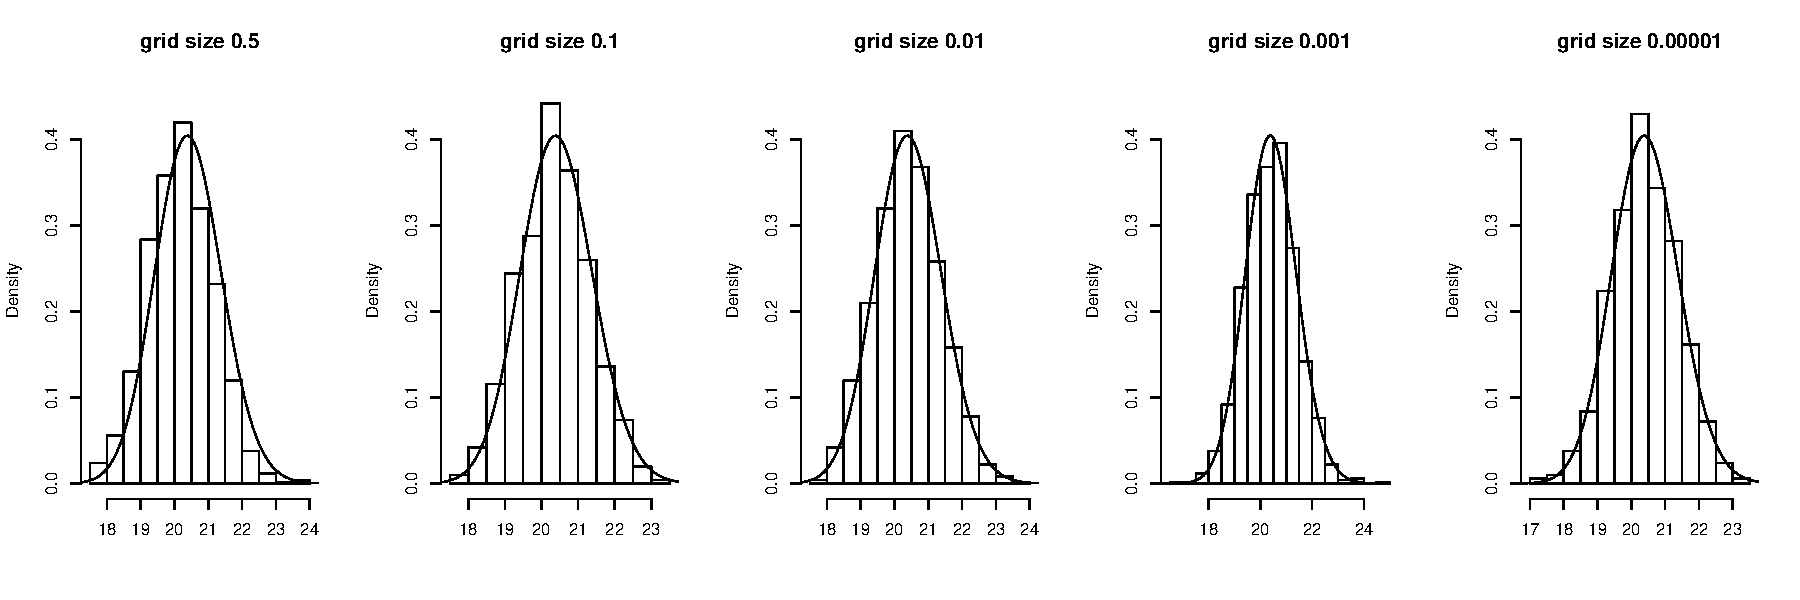
\includegraphics[width=\linewidth]{figure/histograms-1} 

\end{knitrout}
\end{center}

\item The beanplots below show the distribution of $1000$ draws for different grid sizes, as well as the draws from \verb+rgamma+ and the theoretical distribution. I think it is hard to tell how good the approximation is by just looking at the beanplots. The table, however, shows that the posterior interval and posterior probability is closest to the truth at grid sizes of $0.001$ and $0.00001$. \verb+rgamma+ performs similarly to these grid sizes as well.




\begin{knitrout}\footnotesize
\definecolor{shadecolor}{rgb}{0.969, 0.969, 0.969}\color{fgcolor}
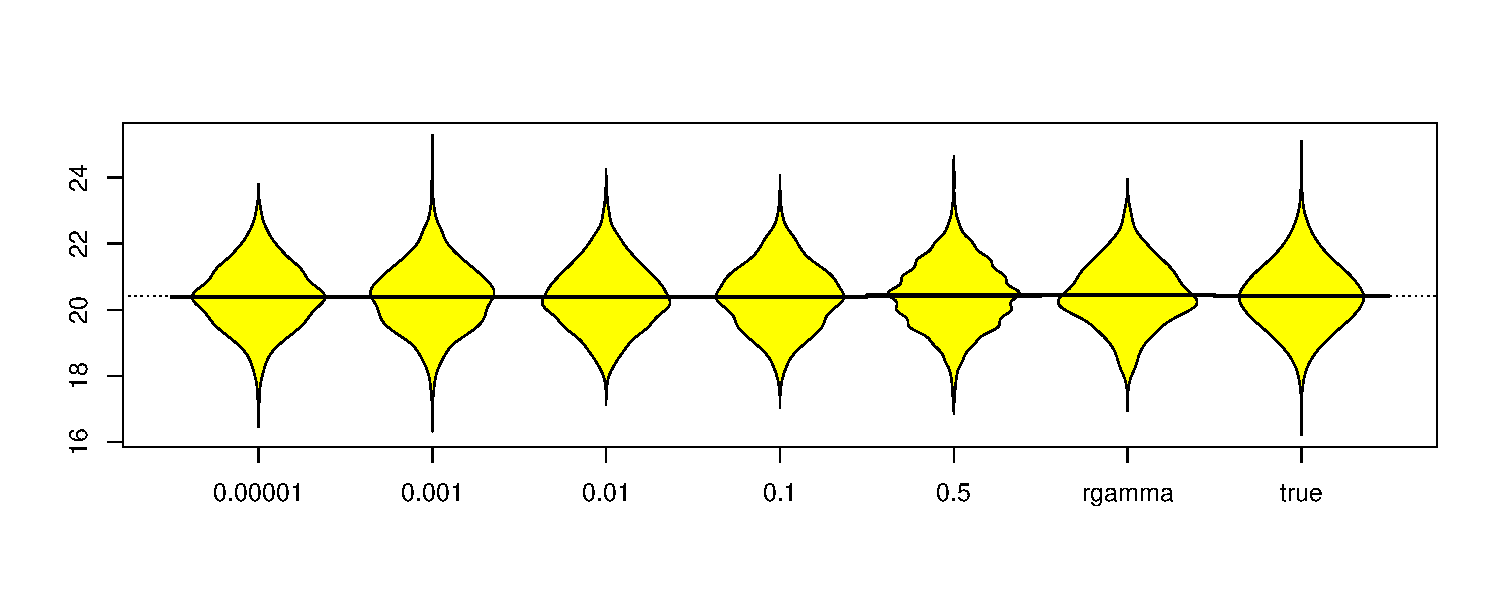
\includegraphics[width=\linewidth]{figure/ciplot-1} 

\end{knitrout}



\begin{table}[H]
\centering
\begin{tabular} {c|c|c|c}
Grid Size & $90\%$ posterior interval & $Pr(10 < x < 20)$ & $Pr(x < 5)$ \\
\hline 
0.5 & (19.0, 22.0) & 0.44 & 0 \\
0.1 & (18.80, 22.10) & 0.36 & 0 \\
0.01 & (18.75, 21.97) & 0.35 & 0 \\
0.001 & (18.81, 22.02) & 0.33 & 0 \\
0.00001 & (18.83, 22.16) & 0.32 & 0 \\
rgamma & (18.86, 22.07) & 0.36 & 0 \\
Theoretical Distribution & (18.84, 22.08) & 0.34 & $\approx 0$ \\
\hline
\end{tabular}
\end{table}

\item I obtained $100$ draws using five different \verb+set.seeds+. For each, I characterized the distribution from which the draws came (a $Gam(429, 21)$). The mean varied between $20.4$ and $20.6$, and the variance was between $0.92$ and $1.12$ (the true mean is $20.43$ and the true variance is $0.97$). I think in many situations, it is adequate to be within $0.2$ of the mean and the variance. So, yes, I think it could be {\it adequate} to characterize a distribution with only $100$ observations. But, it is important to keep in mind the variability we might see in the characteristics of a distribution among different draws of $100$. 

\begin{table} [H]
\centering
\begin{tabular} {c|c|c|c|c|c}
set.seed & $90\%$ posterior interval & $Pr(10 < x < 20)$ & $Pr(x < 5)$ & mean & SD \\
\hline 
set.seed(15) & (18.57, 22.01) & 0.31 & 0 & 20.52 & 0.97 \\
set.seed(16) & (19.06, 21.95) & 0.33 & 0 & 20.51 & 0.97 \\
set.seed(17) & (19.04, 22.05) & 0.36 & 0 & 20.41 & 0.92 \\
set.seed(18) & (19.12, 21.96) & 0.35 & 0 & 20.52 & 0.94 \\
set.seed(19) & (19.24, 21.93) & 0.30 & 0 & 20.59 & 0.93 \\
set.seed(20) & (18.55, 22.07) & 0.31 & 0 & 20.45 & 1.12 \\
Theoretical Distribution & (18.84, 22.08) & 0.34 & $\approx 0$ & 20.43 & 0.97 \\
\hline
\end{tabular}
\end{table}



\vspace{.05in}
\item Using the code from (1), I display the histogram of transformed draws for sample sizes of $10$, $250$, and $10000$. I used the sample size of $10000$ to approximate the mean and variance of these functions of $\lambda$. I am really excited about this, because I don't need to do a mathematical transformation to find information about the distribution for a function of $\lambda$!!! And I don't need to use the Delta Method to approximate the variance of the distribution for a function of $\lambda$! I can simply draw from the distribution of $\lambda$, calculate the desired function of $\lambda$, and use this to approximate the distribution for the function of $\lambda$ (along with mean, variance, and other summary measures).

\begin{table}[H]
\centering
\begin{tabular}{c|c|c}
Transformation & Estimated mean & Estimated Variance \\
\hline
$\frac{\lambda^2}{1-\lambda}$ & -21.47 & 0.97 \\
$log(\lambda)$ & 3.02 & 0.0024 \\
\hline
\end{tabular}
\end{table}

\begin{knitrout}\footnotesize
\definecolor{shadecolor}{rgb}{0.969, 0.969, 0.969}\color{fgcolor}
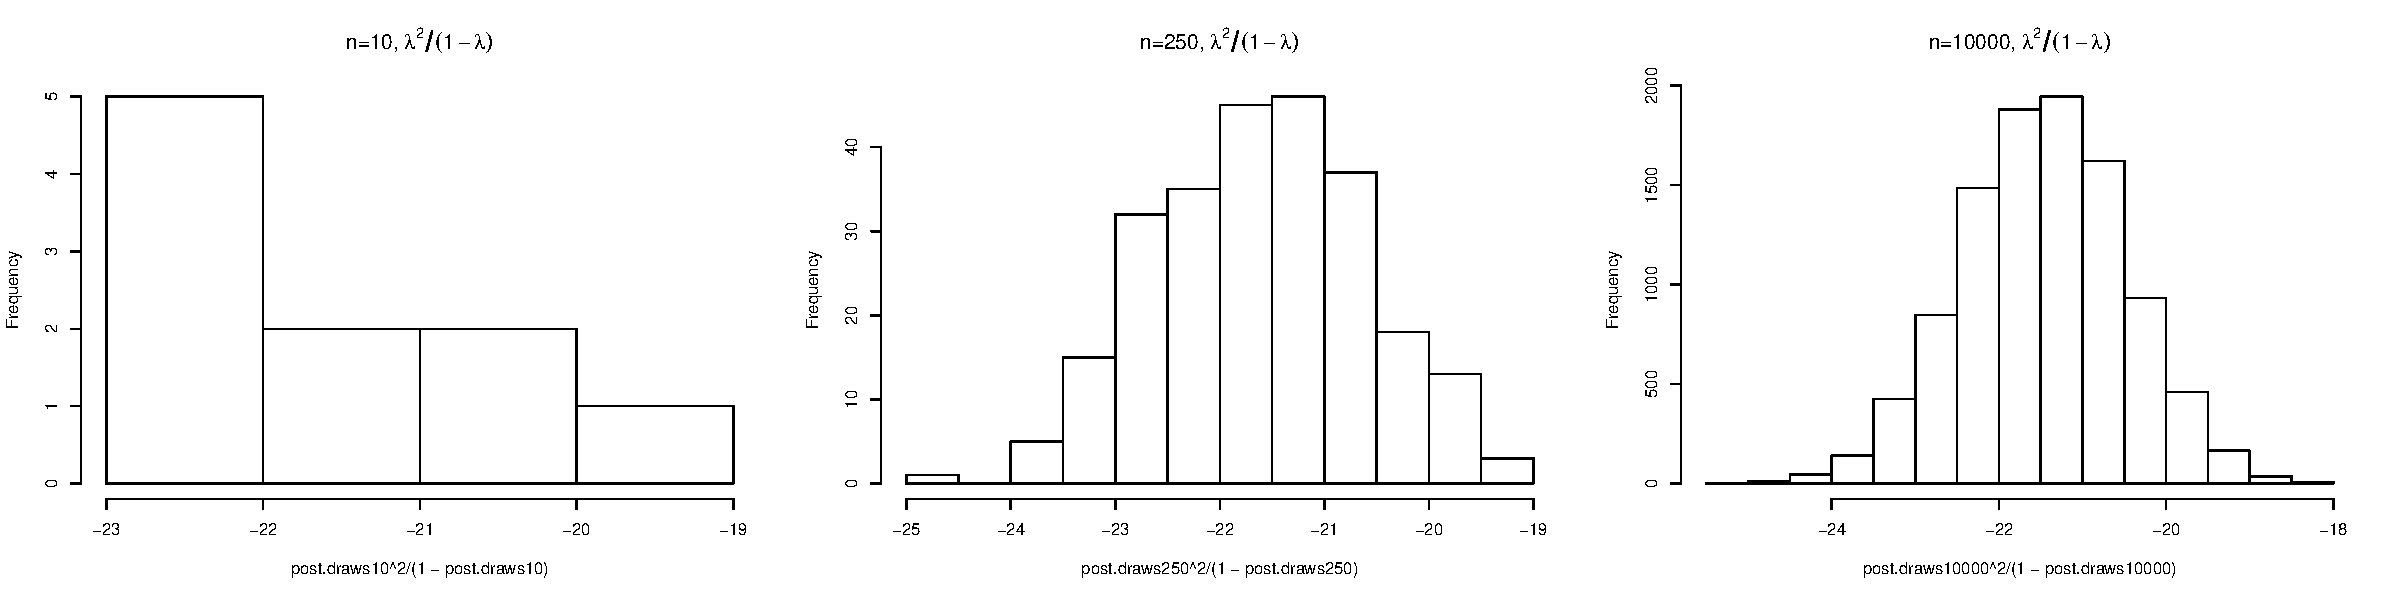
\includegraphics[width=\linewidth]{figure/codetransform-1} 

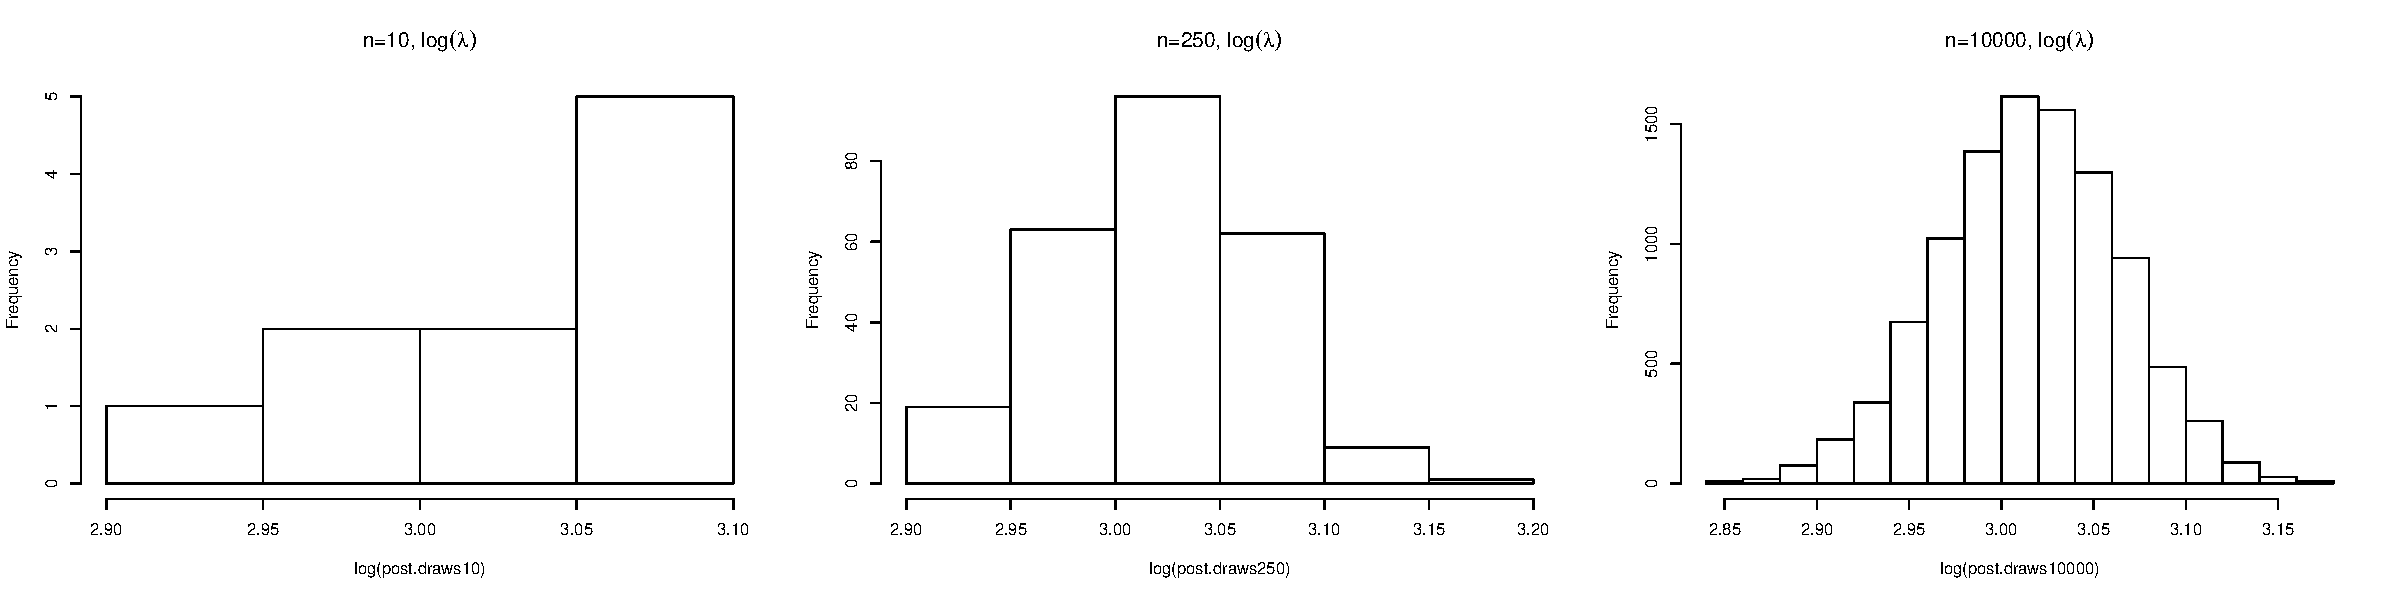
\includegraphics[width=\linewidth]{figure/codetransform-2} 

\end{knitrout}

\item The posterior predictive distribution, $p(\tilde{y}|y)$ is found by integrating the joint distribution of $\tilde{y}, \lambda$, and $y$ over $\lambda$. Since $y$ and $\ytil$ are independent given $\lambda$, it turns out that:
\begin{align*}
p(\tilde{y}|y) &= \int_{\lambda}p(\tilde{y}, \lambda, y) d\lambda = \int_{\lambda}p(\tilde{y}|\lambda, y)p(\lambda|y) d\lambda\\
&= \int_{\lambda}p(\ytil|\lambda)p(\lambda|y) d\lambda
\end{align*}
Recall that in HW3 that the sum of the $20$ observations drawn from a $Poi(20.66)$ distribution was $409$. We then showed that $\lambda|y \sim Gam(429, 21)$.
\begin{align*}
p(\tilde{y}|y) &= \int_{\lambda}\frac{\lambda^{\ytil}e^{-\lambda}}{\tilde{y}!}\frac{\lambda^{428}e^{-21\lambda}21^{429}}{\Gamma(429)} d\lambda \\
&= \int_{\lambda}\frac{\lambda^{\ytil+428}e^{-22\lambda}21^{429}}{\Gamma(\ytil+1)\Gamma(429)} d\lambda \\
&= \frac{21^{429}}{{\Gamma(\ytil+1)\Gamma(429)}}\int_{\lambda}\lambda^{\ytil+428}e^{-22\lambda} d\lambda \\
&= \frac{\Gamma(\ytil+429)21^{429}}{{\Gamma(\ytil+1)\Gamma(429)22^{\ytil+429}}} \\
&= {\ytil+429-1 \choose \ytil}\frac{21}{22}^{429}\frac{1}{22}^{\ytil}
\end{align*}
The posterior predictive distribution is a Negative Binomial distribution with parameters $429$ and $21$, $Neg-bin(429, 21)$.

\item We must assume that future observations are exchangeable with the original data collected. This means that future observations come from the same design and the same process (class notes $9/23$), and will be within the same range as the data collected.

\item The following shows a barplot of $10000$ draws from the $Neg-bin(429, 21)$ distribution.
\begin{center}
\begin{knitrout}\footnotesize
\definecolor{shadecolor}{rgb}{0.969, 0.969, 0.969}\color{fgcolor}
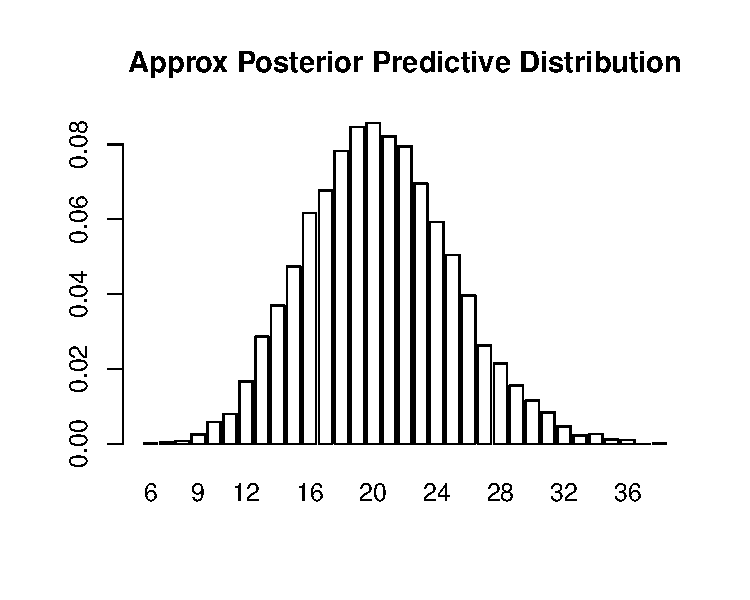
\includegraphics[width=.5\linewidth]{figure/postpreddraws-1} 

\end{knitrout}
\end{center}

\item The following shows the true posterior predictive distribution overlaid on the barplot of $10000$ draws from the previous part. 
\begin{center}
\begin{knitrout}\footnotesize
\definecolor{shadecolor}{rgb}{0.969, 0.969, 0.969}\color{fgcolor}
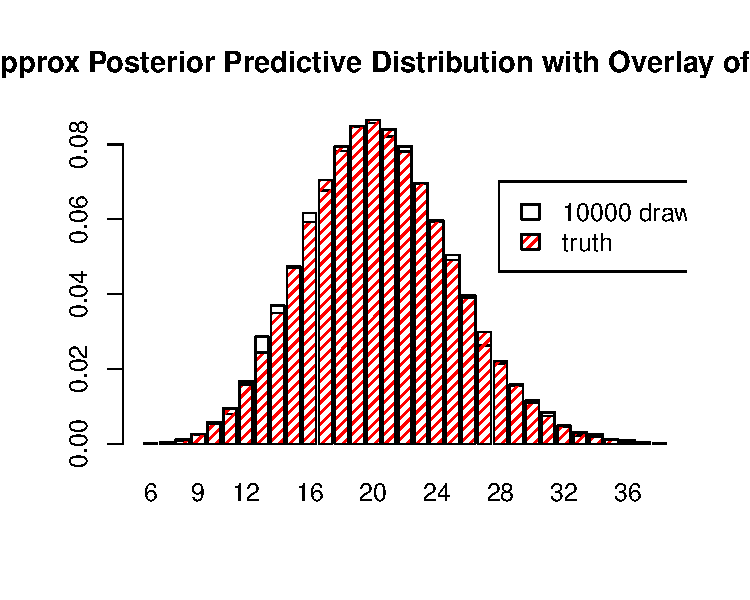
\includegraphics[width=.5\linewidth]{figure/postpreddraws2-1} 

\end{knitrout}
\end{center}

\item The mean of the posterior predictive distribution is $429/21 = 20.43$ and the variance of the posterior predictive distribution is $429/21^2(22) = 21.40$. The mean of the posterior distribution of $\lambda$ ($Gam(429, 21)$) is $429/21 = 20.43$ and the variance of the posterior distribution is $429/21^2 = 0.9728$.\\

I am going to explain this to Chris, mine and Bobby's consulting client from last semester. He has taken $512$, so he has discussed a similar concept in the context of prediction intervals vs. confidence intervals. The posterior distribution for the parameter $\lambda$ describes our knowledge about the possible values of $\lambda$ after incorporating knowledge from the observed data. The mean of the posterior distribution is sometimes used as a point estimate for the parameter $\lambda$ and the spread of the distribution gives us an idea of what values of $\lambda$ we consider to be plausible. So, the larger the spread of the distribution, the more uncertainty there is about the true value of $\lambda$. The posterior predictive distribution, however, reflects two sources of uncertainty. The posterior predictive distribution reflects uncertainty in the true value of $\lambda$ in addition to uncertainty in the value of a future observation. Even if $\lambda$ was known, there is variability that comes from taking random draws from a known distribution. Combining the uncertainty in $\lambda$ and the uncertainty in where the observations will fall around $\lambda$, the posterior predictive distribution has a larger variance. Our best guess for a future observation, however, still lies at our best guess for the mean of the posterior distribution, which is $20.43$.

\item Recall that the prior I set for $\lambda$ was $Gam(20, 1)$. Ignoring observed data, the prior predictive distribution for a single observation is $Neg-Bin(20, 1)$. I solve for the prior predictive distribution analytically below.
\begin{align*}
p(y) &= \frac{p(y|\lambda) p(\lambda)}{p(\lambda|y)} \\
p(y) &= \frac{\frac{\lambda^y \frac{e^{-\lambda}}{y!}e^{-\beta\lambda}\beta^{\alpha}\lambda^{\alpha-1}}{\Gamma(\alpha)}}{\frac{\lambda^{\alpha+y-1}e^{-\lambda(\beta+1)}(\beta+1)^{\alpha+y}}{\Gamma(\alpha+y)}} \\
&= \frac{\lambda^{y+\alpha-1}}{\lambda^{\alpha+y-1}} \frac{\beta^{\alpha}}{(\beta+1)^{\alpha+y}} \frac{e^{-(\beta+1)\lambda}}{e^{-(\beta+1)\lambda}} \frac{\Gamma(\alpha+y)}{y!\Gamma(\alpha)} \\
&= \frac{\beta^{\alpha}}{(\beta+1)^{\alpha+y}}\frac{\Gamma(\alpha+y)}{\Gamma(\alpha)y!} \\
&= {\alpha+y-1 \choose y}(\frac{\beta}{\beta+1})^{\alpha} (\frac{1}{\beta+1})^y \\
&= {20+y-1 \choose y}(\frac{1}{1+1})^{20} (\frac{1}{1+1})^y
\end{align*}

\begin{knitrout}\footnotesize
\definecolor{shadecolor}{rgb}{0.969, 0.969, 0.969}\color{fgcolor}
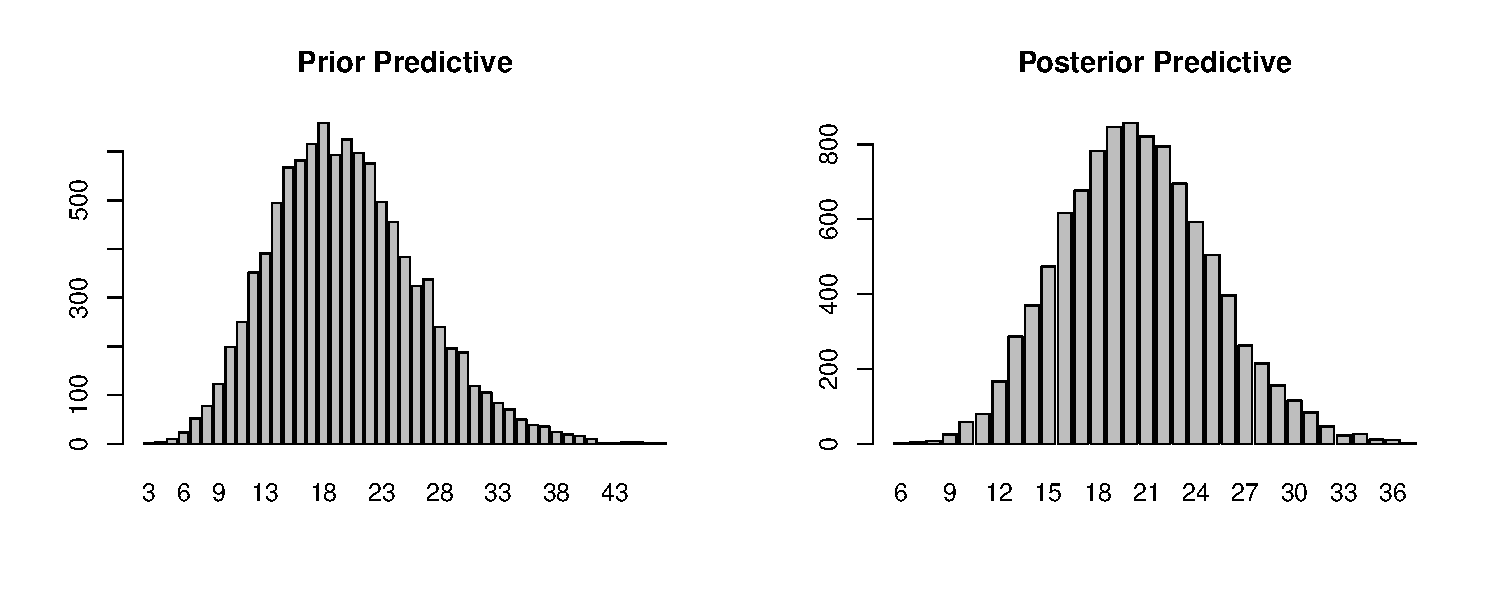
\includegraphics[width=\linewidth]{figure/priorpred-1} 

\end{knitrout}



\begin{table}[H]
\centering
\begin{tabular}{c|c|c|c}
 & $90\%$ interval & Estimated mean & Estimated Variance \\
\hline
Prior predicted & (11, 31) & 19.99 & 6.32 \\
Posterior predicted & (13, 28) & 20.38 & 4.63 \\
\hline
\end{tabular}
\end{table}


The main difference between the prior and posterior predictive distributions in the spread. The prior predictive distribution has a larger variance and a wider range of plausible values than the posterior predictive distribution. The prior predictive distribution is slightly more skewed than the posterior predictive distribution.

\item I drew $1000$ samples of size $20$ from the posterior predictive distribution. $9$ of them are shown below. I played around with using dotplots rather than barplots. The only thing I don't like about them is that I couldn't figure out how to get numbers on the y-axis.

\begin{knitrout}\footnotesize
\definecolor{shadecolor}{rgb}{0.969, 0.969, 0.969}\color{fgcolor}
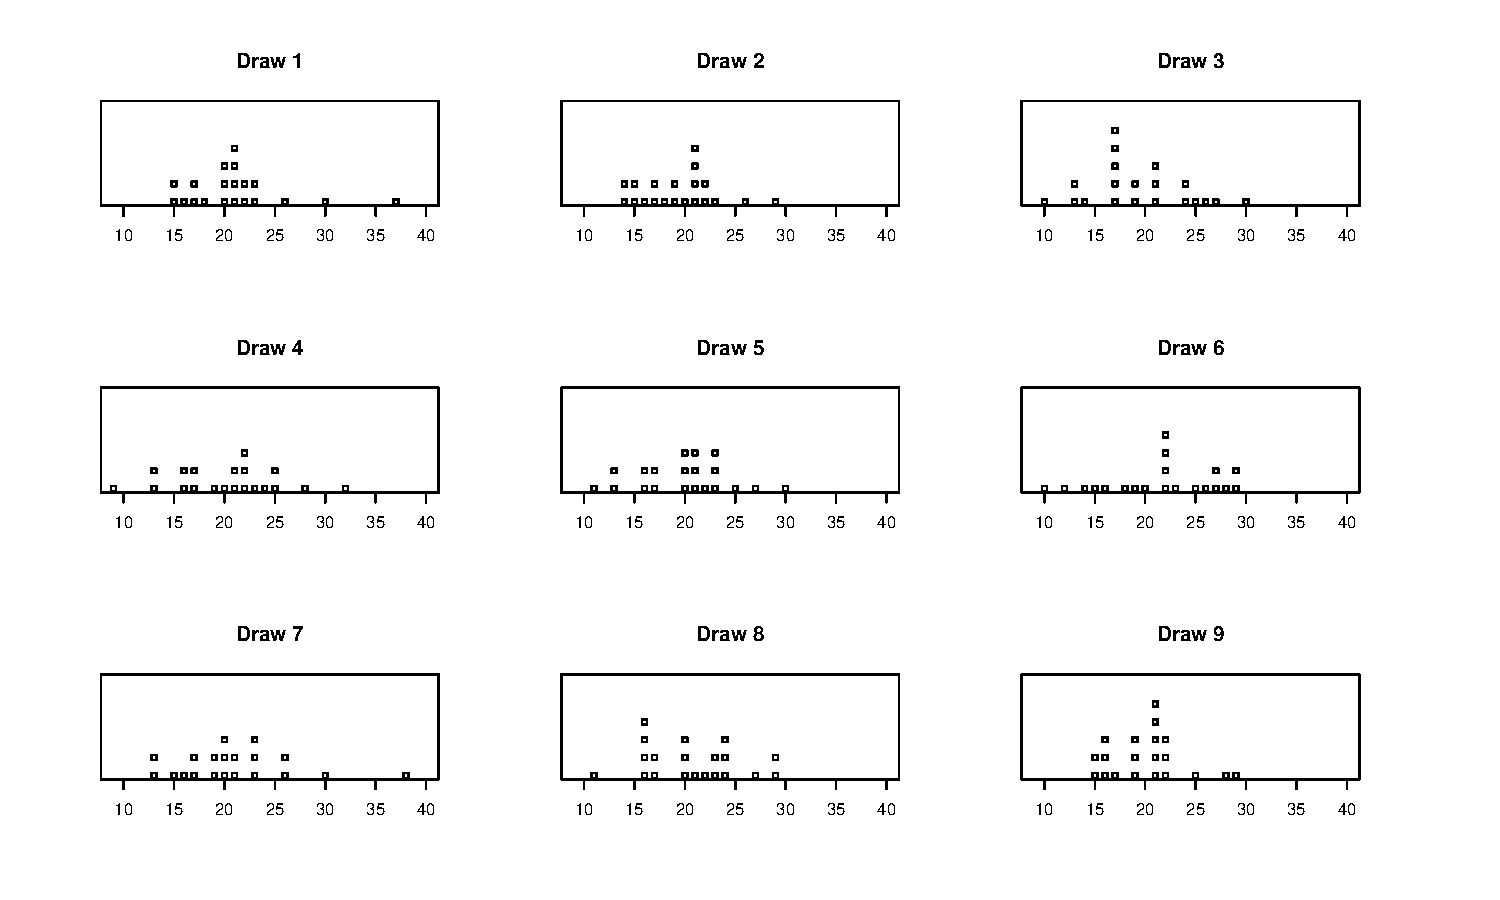
\includegraphics[width=\linewidth]{figure/drawmatrix-1} 

\end{knitrout}

\item The approximate posterior predictive distribution for the sample standard deviation is shown below. The standard deviation observed in the original sample is in the center of the standard deviations found for the posterior predictive samples. I think the fact that the standard deviation from the original sample is right in the middle of the standard deviations from the posterior predictions is somewhat of a coincidence. We assume that the posterior predictions come from the same design and process as the original observations. This means that the summary measure of the original observed draws should be within the same range as what could be observed in the posterior predictions. I investigated further to see where the original sample standard deviation could lie in the posterior predictive distribution for the sample standard deviation. In the following plots, I generated a new sample of size $20$ from a $Poi(20.66)$ distribution. I then found the corresponding posterior predictive distribution ($Neg-Bin(\sum x_i, 21)$), and then I constructed an approximate posterior predictive distribution for the sample standard deviation. The following plots show that the sample standard deviation from the original data can lie anywhere in the posterior predictive distribution.

\begin{center}
\begin{knitrout}\footnotesize
\definecolor{shadecolor}{rgb}{0.969, 0.969, 0.969}\color{fgcolor}
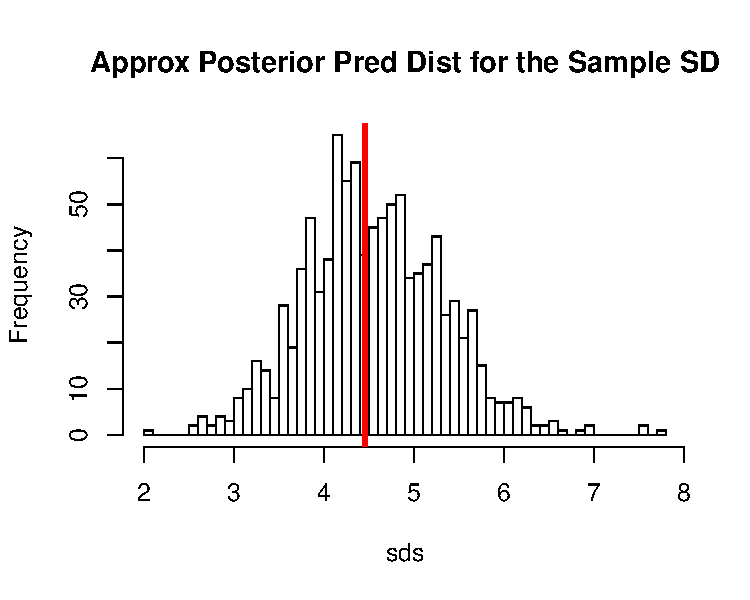
\includegraphics[width=.5\linewidth]{figure/postsds-1} 

\end{knitrout}
\end{center}

\begin{knitrout}\footnotesize
\definecolor{shadecolor}{rgb}{0.969, 0.969, 0.969}\color{fgcolor}
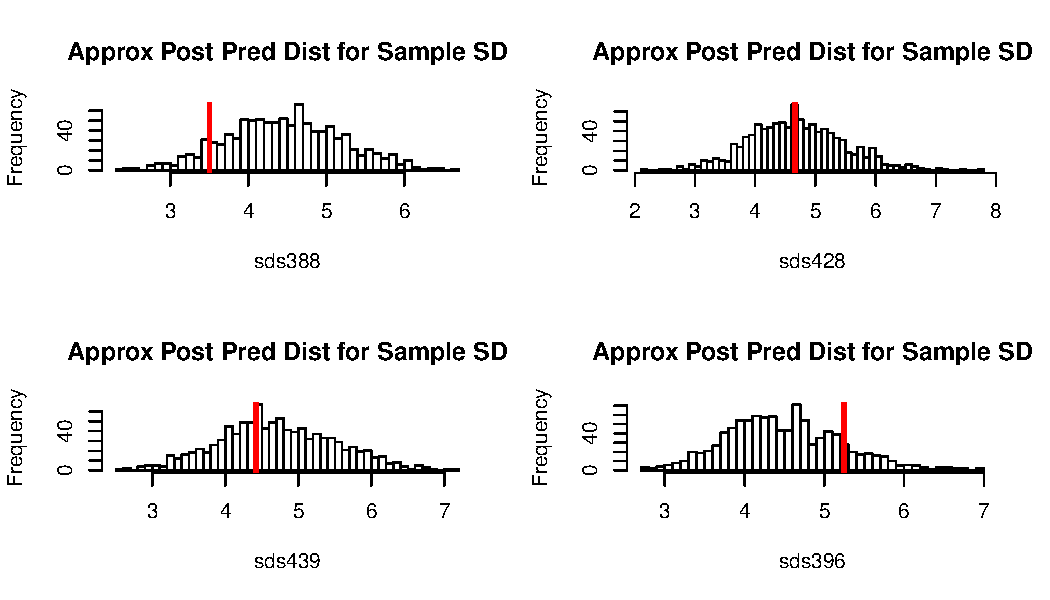
\includegraphics[width=\linewidth]{figure/otherdraws-1} 

\end{knitrout}


\item The approximate posterior predictive distribution for the sample maximum is shown below. The maximum observed in the original sample is in the center of the maximums found for the posterior predictive samples, but again I think this is just coincidence. I did a similar exploration as the previous problem. In the four samples I investigated, the location of the original sample maximum on the histogram of posterior predicted maximums varied; but the original maximum was always within the range of posterior predicted maximums.

\begin{center}
\begin{knitrout}\footnotesize
\definecolor{shadecolor}{rgb}{0.969, 0.969, 0.969}\color{fgcolor}
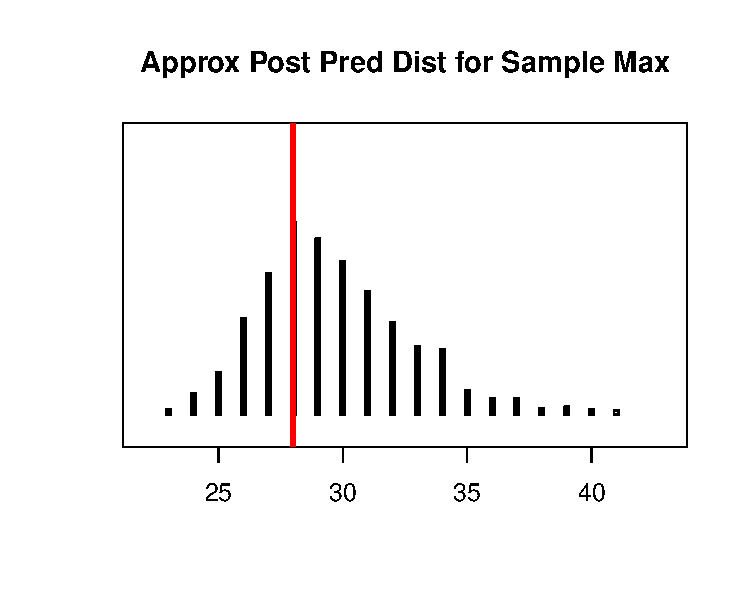
\includegraphics[width=.5\linewidth]{figure/postmax-1} 

\end{knitrout}
\end{center}

\begin{knitrout}\footnotesize
\definecolor{shadecolor}{rgb}{0.969, 0.969, 0.969}\color{fgcolor}
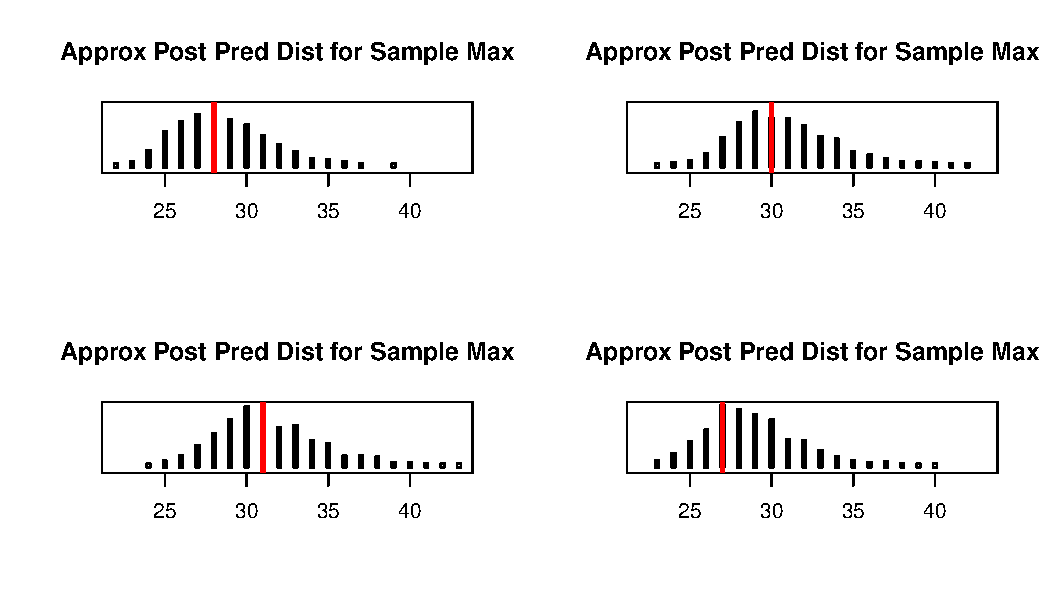
\includegraphics[width=\linewidth]{figure/explore2-1} 

\end{knitrout}


\end{enumerate}

\noindent {\bf \underline{Problem 2}}:

\noindent Consider the regression model,
\begin{align*}
log(salary_i) &= \beta_0+\beta_1I_{male}+\epsilon_i
\end{align*}
where $I_{male}=1$ if male and $0$ otherwise. In this regression model, $\beta_1$ represents the difference in salaries between males and females on the log scale. After backtransforming, $e^{\beta_1}$ represents the multiplicative difference in salaries between males and females. Gelman is thinking about what an appropriate prior for $\beta_1$ would be. If he puts a $Unif(-10, 10)$ prior on $\beta_1$, then this implies that the multiplicative difference in salaries between males and females could range between $e^{-10}\approx\frac{1}{20000}$ and $e^10\approx 20000$, allowing for the possibility that either females have salaries $20000$ times that of males, or males have salaries $20000$ times that of females. These are natural constraints because it would be totally absurd for the gender effect on salary to be more extreme than that. Although an effect size of $10$ doesn't seem very big on the log scale, it actually is big on the original scale. \\

\noindent We can think of a similar example on the logit scale. Consider the regression model,
\begin{align*}
logit(p_i) &= \beta_0+\beta_1I_{male}
\end{align*}
where $I_{male}=1$ if male and $0$ otherwise. For this example, suppose $p_i$ represents the probability of going bankrupt. In this case, $\beta_1$ represents that odds ratio of going bankrupt between males and females. Suppose we put a $(-5, 5)$ prior on $\beta_1$. This would imply that the odds ratio is somewhere between $e^{-5}\approx \frac{1}{150}$ and $e^{5}\approx 150$. This would mean that the odds of females going bankrupt could be $150$ times the odds of males going bankrupt, or the odds of males going bankrupt could be $150$ times the odds of females going bankrupt. To explain what this means on the probability scale, I'll start by assuming the probability of females going bankrupt is $0.2$. That means that the log odds of males going bankrupt is $\beta_1+log(0.2/0.8)$. If $\beta_1=5$, then $5+log(0.2/0.8)=3.61$ and the probabililty of males going bankrupt is $e^{3.61}/(1+e^{3.61})=0.97$. If $\beta_1=-5$, then $-5+log(0.2/0.8)=-6.39$ and the probability of males going bankrupt is $e^{-6.39}/(1+e^{-6.39})=0.0017$. I think Gelman is actually assuming that probability of females going bankrupt is $0.5$. That means that the log odds of males going bankrupt is simply $\beta_1$, and the probability of males going bankrupt is somewhere between $e^{-5}/(1+e^{-5})=0.01$ and $e^{5}/(1+e^{5})=0.99$. This would mean that the probability of males going bankrupt is somewhere between $0.49$ lower or $0.49$ higher than the probability of females going bankrupt. 

\noindent {\bf \underline{Problem 3}}

\begin{enumerate}
\item If $y \sim Expon(\theta)$, then $P(y \geq 100|\theta) = e^{-100\theta}$ from the cdf of the exponential distribution. Below I show that the posterior distribution of $\theta$ given $y \geq 100$ is $Gam(\alpha, \beta+100)$. The mean is $\frac{\alpha}{\beta+100}$ and the variance is $\frac{\alpha}{(\beta+100)^2}$.
\begin{align*}
p(\theta|y\geq 100) &\propto e^{-100\theta} \theta^{\alpha-1} e^{-\beta \theta} \\
&\propto e^{-\theta(100+\beta)}\theta^{\alpha-1}
\end{align*}

\item Below I show that the posterior distribution is $Gam(\alpha+1, \beta+100)$. The posterior mean is now $\frac{\alpha+1}{\beta+100}$ and the posterior variance is now $\frac{\alpha+1}{(\beta+100)^2}$. So, if $y=100$, the posterior mean and the posterior variance are larger than what they would have been if $y \geq 100$.
\begin{align*}
p(\theta|y=100) &\propto \theta e^{-100\theta} \theta^{\alpha-1} e^{-\beta \theta} \\
&\propto e^{-\theta(100+\beta)}\theta^{\alpha+1-1}
\end{align*}

\item Yes, these results do surprise me. First, it surprises me that the posterior mean is higher when $y=100$ compared to $y \geq 100$. If we observe lower values, shouldn't the estimate for $\theta$ be lower? Second, it surprises me that the posterior variance is higher when $y=100$ compared to $y \geq 100$. If $y=100$, we have more information about $y$, and more information generally leads to less uncertainty about $\theta$. As a result, I would have expected the posterior distribution for $\theta$ to have {\it smaller} variance when $y=100$ and {\it larger} variance when $y \geq 100$. 

\end{enumerate}

\noindent {\bf \underline{Problem 4}}

\noindent ``Like Laplace, Fisher insisted that every probability statement depends
on both the knowledge and ignorance that we bring to bear.'' When I was at the ASA Alaska Chapter meeting, the room was full of biometricians from around the state. I had the opportunity to talk to many of them throughout the conference, and one of them told me that just {\it fifteen} years ago, nobody at Fish at Game ever reported confidence intervals (or other measures of uncertainty). They simply reported averages! It's amazing me to that Fisher and Laplace came up with this concept of uncertainty over $100$ years ago and that it took that long to infiltrate research in other disciplines (and it still hasn't in some disciplines). \\

\noindent The author of {\it Willful Ignorance} also talks about statements of probability never being absolutely true or false. But, he says probability statements generally line up with reality and can help inform decisions. This reminds me of the quote that is always thrown around when discussing models, ``All models are wrong, some are useful.'' In statistics, we never actually believe that a model describing some effect is completely correct; we always know that there is process variability that cannot be accounted for by a model. Yet, we assume that models do generally line up with reality and that they can help us to describe relationships and effects. I don't have a lot of experience with how researchers in other disciplines use models. I suspect that they don't fully acknowledge how much uncertainty there is around a fitted model, and they probably put too much stock and belief into one fitted model.\\

\noindent He ends with a philosophical statement about probability being a technique for thinking and drawing conclusions about the world around us. Statistical inference is not a black and white method for making decisive conclusions, it's simply a guide to help researchers understand processes in the world. My consulting client this year told me that he doesn't want to use 'evidence' statements to describe conclusions, he wants to use 'significant' or 'not significant' because that is what his advisor prefers. Making decisive statements about whether a null hypothesis is true or false seems to contradict most of what the author said in this paragraph. Again, I'll say that it seems odd that the ideas in this paragraph were developed so long ago, yet inference in many disciplines developed in a way that contradicts these ideas. I think we are in a really interesting age where people are stepping back and revisiting how probability and inference should be used in practice. It is clearly important for statisticians (and maybe philosophers too!) to continue having discussions with researchers in other disciplines about how results of statistical analyses should be interpreted and what conclusions, if any, can be drawn. \\

\end{doublespacing}
\vspace{0.5in}

{\large \bf R code appendix}
\begin{knitrout}\footnotesize
\definecolor{shadecolor}{rgb}{0.969, 0.969, 0.969}\color{fgcolor}\begin{kframe}
\begin{alltt}
\hlkwd{set.seed}\hlstd{(}\hlnum{15}\hlstd{)}
\hlstd{lambda.draw} \hlkwb{<-} \hlkwd{rgamma}\hlstd{(}\hlnum{1}\hlstd{,} \hlnum{20}\hlstd{,} \hlnum{1}\hlstd{)}
\hlstd{x.vec} \hlkwb{<-} \hlkwd{rpois}\hlstd{(}\hlnum{20}\hlstd{, lambda.draw)}
\hlcom{#sum(x.vec)=409}

\hlstd{post.draws10} \hlkwb{<-} \hlkwd{rgamma}\hlstd{(}\hlnum{10}\hlstd{,} \hlnum{429}\hlstd{,} \hlnum{21}\hlstd{)}
\hlcom{#90\textbackslash{}% posterior interval}
\hlkwd{c}\hlstd{(}\hlkwd{quantile}\hlstd{(post.draws10,} \hlnum{0.05}\hlstd{),} \hlkwd{quantile}\hlstd{(post.draws10,} \hlnum{0.95}\hlstd{))}
\hlcom{#posterior probability of being between 10 and 20}
\hlkwd{require}\hlstd{(mosaic)}
\hlkwd{pdata}\hlstd{(}\hlnum{20}\hlstd{, post.draws10)}\hlopt{-}\hlkwd{pdata}\hlstd{(}\hlnum{10}\hlstd{, post.draws10)}
\hlcom{#posterior probability of being less than 5}
\hlkwd{pdata}\hlstd{(}\hlnum{5}\hlstd{, post.draws10)}

\hlstd{post.draws50} \hlkwb{<-} \hlkwd{rgamma}\hlstd{(}\hlnum{50}\hlstd{,} \hlnum{429}\hlstd{,} \hlnum{21}\hlstd{)}
\hlcom{#90\textbackslash{}% posterior interval}
\hlkwd{c}\hlstd{(}\hlkwd{quantile}\hlstd{(post.draws50,} \hlnum{0.05}\hlstd{),} \hlkwd{quantile}\hlstd{(post.draws50,} \hlnum{0.95}\hlstd{))}
\hlcom{#posterior probability of being between 10 and 20}
\hlkwd{require}\hlstd{(mosaic)}
\hlkwd{pdata}\hlstd{(}\hlnum{20}\hlstd{, post.draws50)}\hlopt{-}\hlkwd{pdata}\hlstd{(}\hlnum{10}\hlstd{, post.draws50)}
\hlcom{#posterior probability of being less than 5}
\hlkwd{pdata}\hlstd{(}\hlnum{5}\hlstd{, post.draws50)}

\hlstd{post.draws100} \hlkwb{<-} \hlkwd{rgamma}\hlstd{(}\hlnum{100}\hlstd{,} \hlnum{429}\hlstd{,} \hlnum{21}\hlstd{)}
\hlcom{#90\textbackslash{}% posterior interval}
\hlkwd{c}\hlstd{(}\hlkwd{quantile}\hlstd{(post.draws100,} \hlnum{0.05}\hlstd{),} \hlkwd{quantile}\hlstd{(post.draws100,} \hlnum{0.95}\hlstd{))}
\hlcom{#posterior probability of being between 10 and 20}
\hlkwd{require}\hlstd{(mosaic)}
\hlkwd{pdata}\hlstd{(}\hlnum{20}\hlstd{, post.draws100)}\hlopt{-}\hlkwd{pdata}\hlstd{(}\hlnum{10}\hlstd{, post.draws100)}
\hlcom{#posterior probability of being less than 5}
\hlkwd{pdata}\hlstd{(}\hlnum{5}\hlstd{, post.draws100)}

\hlstd{post.draws250} \hlkwb{<-} \hlkwd{rgamma}\hlstd{(}\hlnum{250}\hlstd{,} \hlnum{429}\hlstd{,} \hlnum{21}\hlstd{)}
\hlcom{#90\textbackslash{}% posterior interval}
\hlkwd{c}\hlstd{(}\hlkwd{quantile}\hlstd{(post.draws250,} \hlnum{0.05}\hlstd{),} \hlkwd{quantile}\hlstd{(post.draws250,} \hlnum{0.95}\hlstd{))}
\hlcom{#posterior probability of being between 10 and 20}
\hlkwd{require}\hlstd{(mosaic)}
\hlkwd{pdata}\hlstd{(}\hlnum{20}\hlstd{, post.draws250)}\hlopt{-}\hlkwd{pdata}\hlstd{(}\hlnum{10}\hlstd{, post.draws250)}
\hlcom{#posterior probability of being less than 5}
\hlkwd{pdata}\hlstd{(}\hlnum{5}\hlstd{, post.draws250)}

\hlstd{post.draws1000} \hlkwb{<-} \hlkwd{rgamma}\hlstd{(}\hlnum{1000}\hlstd{,} \hlnum{429}\hlstd{,} \hlnum{21}\hlstd{)}
\hlcom{#90\textbackslash{}% posterior interval}
\hlkwd{c}\hlstd{(}\hlkwd{quantile}\hlstd{(post.draws1000,} \hlnum{0.05}\hlstd{),} \hlkwd{quantile}\hlstd{(post.draws1000,} \hlnum{0.95}\hlstd{))}
\hlcom{#posterior probability of being between 10 and 20}
\hlkwd{require}\hlstd{(mosaic)}
\hlkwd{pdata}\hlstd{(}\hlnum{20}\hlstd{, post.draws1000)}\hlopt{-}\hlkwd{pdata}\hlstd{(}\hlnum{10}\hlstd{, post.draws1000)}
\hlcom{#posterior probability of being less than 5}
\hlkwd{pdata}\hlstd{(}\hlnum{5}\hlstd{, post.draws1000)}

\hlstd{post.draws10000} \hlkwb{<-} \hlkwd{rgamma}\hlstd{(}\hlnum{10000}\hlstd{,} \hlnum{429}\hlstd{,} \hlnum{21}\hlstd{)}
\hlcom{#90\textbackslash{}% posterior interval}
\hlkwd{c}\hlstd{(}\hlkwd{quantile}\hlstd{(post.draws10000,} \hlnum{0.05}\hlstd{),} \hlkwd{quantile}\hlstd{(post.draws10000,} \hlnum{0.95}\hlstd{))}
\hlcom{#posterior probability of being between 10 and 20}
\hlkwd{require}\hlstd{(mosaic)}
\hlkwd{pdata}\hlstd{(}\hlnum{20}\hlstd{, post.draws10000)}\hlopt{-}\hlkwd{pdata}\hlstd{(}\hlnum{10}\hlstd{, post.draws10000)}
\hlcom{#posterior probability of being less than 5}
\hlkwd{pdata}\hlstd{(}\hlnum{5}\hlstd{, post.draws10000)}
\end{alltt}
\end{kframe}
\end{knitrout}

\begin{knitrout}\footnotesize
\definecolor{shadecolor}{rgb}{0.969, 0.969, 0.969}\color{fgcolor}\begin{kframe}
\begin{alltt}
\hlcom{#function to calculate posterior probabilities}
\hlstd{posterior} \hlkwb{<-} \hlkwa{function}\hlstd{(}\hlkwc{x}\hlstd{)\{}
  \hlkwd{dgamma}\hlstd{(x,} \hlnum{429}\hlstd{,} \hlnum{21}\hlstd{)}
\hlstd{\}}

\hlcom{#possible x values}
\hlcom{#use small grid size}
\hlstd{xsmall} \hlkwb{<-} \hlkwd{seq}\hlstd{(}\hlnum{15}\hlstd{,} \hlnum{25}\hlstd{,} \hlnum{.00001}\hlstd{)}

\hlcom{##sample x with probability proportional to height of function within that grid}
\hlkwd{set.seed}\hlstd{(}\hlnum{17}\hlstd{)}
\hlstd{grid.draws} \hlkwb{<-} \hlkwd{sample}\hlstd{(xsmall,} \hlnum{1000}\hlstd{,} \hlkwc{prob}\hlstd{=}\hlkwd{posterior}\hlstd{(xsmall))}

\hlcom{#plot draws with posterior overlaid}
\hlcom{#hist(grid.draws, freq=F, main="grid size 0.00001")}
\hlcom{#lines(xsmall, posterior(xsmall))}
\end{alltt}
\end{kframe}
\end{knitrout}

\begin{knitrout}\footnotesize
\definecolor{shadecolor}{rgb}{0.969, 0.969, 0.969}\color{fgcolor}\begin{kframe}
\begin{alltt}
\hlkwd{set.seed}\hlstd{(}\hlnum{18}\hlstd{)}
\hlstd{xmiddle} \hlkwb{<-} \hlkwd{seq}\hlstd{(}\hlnum{15}\hlstd{,} \hlnum{25}\hlstd{,} \hlnum{0.1}\hlstd{)}

\hlkwd{par}\hlstd{(}\hlkwc{mfrow}\hlstd{=}\hlkwd{c}\hlstd{(}\hlnum{1}\hlstd{,}\hlnum{5}\hlstd{))}

\hlcom{#try a big grid=0.5}
\hlstd{xbig} \hlkwb{<-} \hlkwd{seq}\hlstd{(}\hlnum{15}\hlstd{,} \hlnum{25}\hlstd{,} \hlnum{0.5}\hlstd{)}
\hlstd{grid.drawsbig} \hlkwb{<-} \hlkwd{sample}\hlstd{(xbig,} \hlkwc{size}\hlstd{=}\hlnum{1000}\hlstd{,} \hlkwc{replace} \hlstd{=} \hlnum{TRUE}\hlstd{,}
                            \hlkwc{prob} \hlstd{=} \hlkwd{posterior}\hlstd{(xbig))}
\hlkwd{hist}\hlstd{(grid.drawsbig,} \hlkwc{freq}\hlstd{=F,} \hlkwc{main}\hlstd{=}\hlstr{"grid size 0.5"}\hlstd{,} \hlkwc{xlab}\hlstd{=}\hlstr{""}\hlstd{,} \hlkwc{ylim}\hlstd{=}\hlkwd{c}\hlstd{(}\hlnum{0}\hlstd{,} \hlnum{0.45}\hlstd{))}
\hlkwd{lines}\hlstd{(xmiddle,} \hlkwd{posterior}\hlstd{(xmiddle))}

\hlcom{#try a middle grid=0.1}
\hlstd{xmiddle} \hlkwb{<-} \hlkwd{seq}\hlstd{(}\hlnum{15}\hlstd{,} \hlnum{25}\hlstd{,} \hlnum{0.1}\hlstd{)}
\hlstd{grid.drawsmiddle} \hlkwb{<-} \hlkwd{sample}\hlstd{(xmiddle,} \hlnum{1000}\hlstd{,} \hlkwc{replace}\hlstd{=}\hlnum{TRUE}\hlstd{,} \hlkwc{prob}\hlstd{=}\hlkwd{posterior}\hlstd{(xmiddle))}
\hlkwd{hist}\hlstd{(grid.drawsmiddle,} \hlkwc{freq}\hlstd{=F,} \hlkwc{main}\hlstd{=}\hlstr{"grid size 0.1"}\hlstd{,} \hlkwc{xlab}\hlstd{=}\hlstr{""}\hlstd{,} \hlkwc{ylim}\hlstd{=}\hlkwd{c}\hlstd{(}\hlnum{0}\hlstd{,} \hlnum{0.45}\hlstd{))}
\hlkwd{lines}\hlstd{(xmiddle,} \hlkwd{posterior}\hlstd{(xmiddle))}

\hlcom{#try another middle grid=0.01}
\hlstd{xmid} \hlkwb{<-} \hlkwd{seq}\hlstd{(}\hlnum{15}\hlstd{,} \hlnum{25}\hlstd{,} \hlnum{0.01}\hlstd{)}
\hlstd{grid.drawsmid} \hlkwb{<-} \hlkwd{sample}\hlstd{(xmid,} \hlnum{1000}\hlstd{,} \hlkwc{replace}\hlstd{=}\hlnum{TRUE}\hlstd{,} \hlkwc{prob}\hlstd{=}\hlkwd{posterior}\hlstd{(xmid))}
\hlkwd{hist}\hlstd{(grid.drawsmid,} \hlkwc{freq}\hlstd{=F,} \hlkwc{main}\hlstd{=}\hlstr{"grid size 0.01"}\hlstd{,} \hlkwc{xlab}\hlstd{=}\hlstr{""}\hlstd{,} \hlkwc{ylim}\hlstd{=}\hlkwd{c}\hlstd{(}\hlnum{0}\hlstd{,} \hlnum{0.45}\hlstd{))}
\hlkwd{lines}\hlstd{(xmiddle,} \hlkwd{posterior}\hlstd{(xmiddle))}

\hlcom{#try another middle grid=0.001}
\hlstd{xmid2} \hlkwb{<-} \hlkwd{seq}\hlstd{(}\hlnum{15}\hlstd{,} \hlnum{25}\hlstd{,} \hlnum{0.001}\hlstd{)}
\hlstd{grid.drawsmid2} \hlkwb{<-} \hlkwd{sample}\hlstd{(xmid2,} \hlnum{1000}\hlstd{,} \hlkwc{replace}\hlstd{=}\hlnum{TRUE}\hlstd{,} \hlkwc{prob}\hlstd{=}\hlkwd{posterior}\hlstd{(xmid2))}
\hlkwd{hist}\hlstd{(grid.drawsmid2,} \hlkwc{freq}\hlstd{=F,} \hlkwc{main}\hlstd{=}\hlstr{"grid size 0.001"}\hlstd{,} \hlkwc{xlab}\hlstd{=}\hlstr{""}\hlstd{,} \hlkwc{ylim}\hlstd{=}\hlkwd{c}\hlstd{(}\hlnum{0}\hlstd{,} \hlnum{0.45}\hlstd{))}
\hlkwd{lines}\hlstd{(xmiddle,} \hlkwd{posterior}\hlstd{(xmiddle))}

\hlcom{#grid size=0.00001}
\hlkwd{hist}\hlstd{(grid.draws,} \hlkwc{freq}\hlstd{=F,} \hlkwc{main}\hlstd{=}\hlstr{"grid size 0.00001"}\hlstd{,} \hlkwc{xlab}\hlstd{=}\hlstr{""}\hlstd{,} \hlkwc{ylim}\hlstd{=}\hlkwd{c}\hlstd{(}\hlnum{0}\hlstd{,} \hlnum{0.45}\hlstd{))}
\hlkwd{lines}\hlstd{(xmiddle,} \hlkwd{posterior}\hlstd{(xmiddle))}

\hlcom{#compare to rgamma}
\hlcom{#hist(rgamma(1000, 429, 21), freq=F, xlab="", ylim=c(0, 0.45))}
\hlcom{#lines(xmiddle, posterior(xmiddle))}
\end{alltt}
\end{kframe}
\end{knitrout}

\begin{knitrout}\footnotesize
\definecolor{shadecolor}{rgb}{0.969, 0.969, 0.969}\color{fgcolor}\begin{kframe}
\begin{alltt}
\hlstd{post.draws1000} \hlkwb{<-} \hlkwd{rgamma}\hlstd{(}\hlnum{1000}\hlstd{,} \hlnum{429}\hlstd{,} \hlnum{21}\hlstd{)}
\hlcom{#90\textbackslash{}% posterior interval}
\hlkwd{c}\hlstd{(}\hlkwd{quantile}\hlstd{(post.draws1000,} \hlnum{0.05}\hlstd{),} \hlkwd{quantile}\hlstd{(post.draws1000,} \hlnum{0.95}\hlstd{))}
\hlcom{#posterior probability of being between 10 and 20}
\hlkwd{require}\hlstd{(mosaic)}
\hlkwd{pdata}\hlstd{(}\hlnum{20}\hlstd{, post.draws1000)}\hlopt{-}\hlkwd{pdata}\hlstd{(}\hlnum{10}\hlstd{, post.draws1000)}
\hlcom{#posterior probability of being less than 5}
\hlkwd{pdata}\hlstd{(}\hlnum{5}\hlstd{, post.draws1000)}

\hlcom{#grid.draws=0.00001}
\hlcom{#90\textbackslash{}% posterior interval}
\hlkwd{c}\hlstd{(}\hlkwd{quantile}\hlstd{(grid.draws,} \hlnum{0.05}\hlstd{),} \hlkwd{quantile}\hlstd{(grid.draws,} \hlnum{0.95}\hlstd{))}
\hlcom{#posterior probability of being between 10 and 20}
\hlkwd{pdata}\hlstd{(}\hlnum{20}\hlstd{, grid.draws)}\hlopt{-}\hlkwd{pdata}\hlstd{(}\hlnum{10}\hlstd{, grid.draws)}
\hlcom{#posterior probability of being less than 5}
\hlkwd{pdata}\hlstd{(}\hlnum{5}\hlstd{, grid.draws)}

\hlcom{#mid=0.001}
\hlcom{#90\textbackslash{}% posterior interval}
\hlkwd{c}\hlstd{(}\hlkwd{quantile}\hlstd{(grid.drawsmid2,} \hlnum{0.05}\hlstd{),} \hlkwd{quantile}\hlstd{(grid.drawsmid2,} \hlnum{0.95}\hlstd{))}
\hlcom{#posterior probability of being between 10 and 20}
\hlkwd{pdata}\hlstd{(}\hlnum{20}\hlstd{, grid.drawsmid2)}\hlopt{-}\hlkwd{pdata}\hlstd{(}\hlnum{10}\hlstd{, grid.drawsmid2)}
\hlcom{#posterior probability of being less than 5}
\hlkwd{pdata}\hlstd{(}\hlnum{5}\hlstd{, grid.drawsmid2)}

\hlcom{#middle=0.1}
\hlcom{#90\textbackslash{}% posterior interval}
\hlkwd{c}\hlstd{(}\hlkwd{quantile}\hlstd{(grid.drawsmiddle,} \hlnum{0.05}\hlstd{),} \hlkwd{quantile}\hlstd{(grid.drawsmiddle,} \hlnum{0.95}\hlstd{))}
\hlcom{#posterior probability of being between 10 and 20}
\hlkwd{pdata}\hlstd{(}\hlnum{20}\hlstd{, grid.drawsmiddle)}\hlopt{-}\hlkwd{pdata}\hlstd{(}\hlnum{10}\hlstd{, grid.drawsmiddle)}
\hlcom{#posterior probability of being less than 5}
\hlkwd{pdata}\hlstd{(}\hlnum{5}\hlstd{, grid.drawsmiddle)}

\hlcom{#mid=0.01}
\hlcom{#90\textbackslash{}% posterior interval}
\hlkwd{c}\hlstd{(}\hlkwd{quantile}\hlstd{(grid.drawsmid,} \hlnum{0.05}\hlstd{),} \hlkwd{quantile}\hlstd{(grid.drawsmid,} \hlnum{0.95}\hlstd{))}
\hlcom{#posterior probability of being between 10 and 20}
\hlkwd{pdata}\hlstd{(}\hlnum{20}\hlstd{, grid.drawsmid)}\hlopt{-}\hlkwd{pdata}\hlstd{(}\hlnum{10}\hlstd{, grid.drawsmid)}
\hlcom{#posterior probability of being less than 5}
\hlkwd{pdata}\hlstd{(}\hlnum{5}\hlstd{, grid.drawsmid)}

\hlcom{#big=0.5}
\hlcom{#90\textbackslash{}% posterior interval}
\hlkwd{c}\hlstd{(}\hlkwd{quantile}\hlstd{(grid.drawsbig,} \hlnum{0.05}\hlstd{),} \hlkwd{quantile}\hlstd{(grid.drawsbig,} \hlnum{0.95}\hlstd{))}
\hlcom{#posterior probability of being between 10 and 20}
\hlkwd{pdata}\hlstd{(}\hlnum{20}\hlstd{, grid.drawsbig)}\hlopt{-}\hlkwd{pdata}\hlstd{(}\hlnum{10}\hlstd{, grid.drawsbig)}
\hlcom{#posterior probability of being less than 5}
\hlkwd{pdata}\hlstd{(}\hlnum{5}\hlstd{, grid.drawsbig)}
\end{alltt}
\end{kframe}
\end{knitrout}

\begin{knitrout}\footnotesize
\definecolor{shadecolor}{rgb}{0.969, 0.969, 0.969}\color{fgcolor}\begin{kframe}
\begin{alltt}
\hlstd{a} \hlkwb{<-} \hlkwd{c}\hlstd{(}\hlkwd{rep}\hlstd{(}\hlstr{"0.5"}\hlstd{,}\hlnum{1000}\hlstd{),} \hlkwd{rep}\hlstd{(}\hlstr{"0.1"}\hlstd{,}\hlnum{1000}\hlstd{),} \hlkwd{rep}\hlstd{(}\hlstr{"0.01"}\hlstd{,} \hlnum{1000}\hlstd{),} \hlkwd{rep}\hlstd{(}\hlstr{"0.001"}\hlstd{,} \hlnum{1000}\hlstd{),} \hlkwd{rep}\hlstd{(}\hlstr{"0.00001"}\hlstd{,} \hlnum{1000}\hlstd{),} \hlkwd{rep}\hlstd{(}\hlstr{"rgamma"}\hlstd{,}\hlnum{1000}\hlstd{),} \hlkwd{rep}\hlstd{(}\hlstr{"true"}\hlstd{,} \hlnum{10000}\hlstd{))}

\hlstd{test} \hlkwb{<-} \hlkwd{c}\hlstd{(}\hlkwd{as.numeric}\hlstd{(grid.drawsbig), grid.drawsmiddle, grid.drawsmid, grid.drawsmid2, grid.draws, post.draws1000,} \hlkwd{rgamma}\hlstd{(}\hlnum{10000}\hlstd{,} \hlnum{429}\hlstd{,} \hlnum{21}\hlstd{))}
\hlstd{beansetup} \hlkwb{<-} \hlkwd{cbind.data.frame}\hlstd{(test, a)}
\hlkwd{require}\hlstd{(beanplot,} \hlkwc{quietly}\hlstd{=T)}
\hlkwd{beanplot}\hlstd{(test}\hlopt{~}\hlstd{a,} \hlkwc{data}\hlstd{=beansetup,} \hlkwc{log}\hlstd{=}\hlstr{""}\hlstd{,} \hlkwc{col}\hlstd{=}\hlnum{7}\hlstd{,} \hlkwc{what} \hlstd{=} \hlkwd{c}\hlstd{(}\hlnum{1}\hlstd{,}\hlnum{1}\hlstd{,}\hlnum{1}\hlstd{,}\hlnum{0}\hlstd{))}
\end{alltt}
\end{kframe}
\end{knitrout}

\begin{knitrout}\footnotesize
\definecolor{shadecolor}{rgb}{0.969, 0.969, 0.969}\color{fgcolor}\begin{kframe}
\begin{alltt}
\hlstd{post.draws100} \hlkwb{<-} \hlkwd{rgamma}\hlstd{(}\hlnum{100}\hlstd{,} \hlnum{429}\hlstd{,} \hlnum{21}\hlstd{)}
\hlcom{#90\textbackslash{}% posterior interval}
\hlkwd{c}\hlstd{(}\hlkwd{quantile}\hlstd{(post.draws100,} \hlnum{0.05}\hlstd{),} \hlkwd{quantile}\hlstd{(post.draws100,} \hlnum{0.95}\hlstd{))}
\hlcom{#posterior probability of being between 10 and 20}
\hlkwd{pdata}\hlstd{(}\hlnum{20}\hlstd{, post.draws100)}\hlopt{-}\hlkwd{pdata}\hlstd{(}\hlnum{10}\hlstd{, post.draws100)}
\hlcom{#posterior probability of being less than 5}
\hlkwd{pdata}\hlstd{(}\hlnum{5}\hlstd{, post.draws100)}

\hlkwd{set.seed}\hlstd{(}\hlnum{15}\hlstd{)}
\hlkwd{set.seed}\hlstd{(}\hlnum{16}\hlstd{)}
\hlkwd{set.seed}\hlstd{(}\hlnum{17}\hlstd{)}
\hlkwd{set.seed}\hlstd{(}\hlnum{18}\hlstd{)}
\hlkwd{set.seed}\hlstd{(}\hlnum{19}\hlstd{)}
\hlkwd{set.seed}\hlstd{(}\hlnum{20}\hlstd{)}

\hlkwd{mean}\hlstd{(post.draws100)}
\hlkwd{sd}\hlstd{(post.draws100)}
\end{alltt}
\end{kframe}
\end{knitrout}

\begin{knitrout}\footnotesize
\definecolor{shadecolor}{rgb}{0.969, 0.969, 0.969}\color{fgcolor}\begin{kframe}
\begin{alltt}
\hlkwd{par}\hlstd{(}\hlkwc{mfrow}\hlstd{=}\hlkwd{c}\hlstd{(}\hlnum{1}\hlstd{,}\hlnum{3}\hlstd{))}

\hlkwd{hist}\hlstd{(post.draws10}\hlopt{^}\hlnum{2}\hlopt{/}\hlstd{(}\hlnum{1}\hlopt{-}\hlstd{post.draws10),} \hlkwc{main}\hlstd{=}\hlkwd{expression}\hlstd{(}\hlkwd{paste}\hlstd{(}\hlstr{"n=10, "}\hlstd{, lambda}\hlopt{^}\hlnum{2}\hlopt{/}\hlstd{(}\hlnum{1}\hlopt{-}\hlstd{lambda))))}
\hlcom{#hist(post.draws50^2/(1-post.draws50), main=expression(paste("n=50, ", lambda^2/(1-lambda))))}
\hlcom{#hist(post.draws100^2/(1-post.draws100), main=expression(paste("n=100, ", lambda^2/(1-lambda))))}
\hlkwd{hist}\hlstd{(post.draws250}\hlopt{^}\hlnum{2}\hlopt{/}\hlstd{(}\hlnum{1}\hlopt{-}\hlstd{post.draws250),} \hlkwc{main}\hlstd{=}\hlkwd{expression}\hlstd{(}\hlkwd{paste}\hlstd{(}\hlstr{"n=250, "}\hlstd{, lambda}\hlopt{^}\hlnum{2}\hlopt{/}\hlstd{(}\hlnum{1}\hlopt{-}\hlstd{lambda))))}
\hlcom{#hist(post.draws1000^2/(1-post.draws1000), main=expression(paste("n=1000, ", lambda^2/(1-lambda))))}
\hlkwd{hist}\hlstd{(post.draws10000}\hlopt{^}\hlnum{2}\hlopt{/}\hlstd{(}\hlnum{1}\hlopt{-}\hlstd{post.draws10000),} \hlkwc{main}\hlstd{=}\hlkwd{expression}\hlstd{(}\hlkwd{paste}\hlstd{(}\hlstr{"n=10000, "}\hlstd{, lambda}\hlopt{^}\hlnum{2}\hlopt{/}\hlstd{(}\hlnum{1}\hlopt{-}\hlstd{lambda))))}

\hlkwd{hist}\hlstd{(}\hlkwd{log}\hlstd{(post.draws10),} \hlkwc{main}\hlstd{=}\hlkwd{expression}\hlstd{(}\hlkwd{paste}\hlstd{(}\hlstr{"n=10, "}\hlstd{,} \hlkwd{log}\hlstd{(lambda))))}
\hlcom{#hist(log(post.draws50), main=expression(paste("n=50, ", log(lambda))))}
\hlcom{#hist(log(post.draws100), main=expression(paste("n=100, ", log(lambda))))}
\hlkwd{hist}\hlstd{(}\hlkwd{log}\hlstd{(post.draws250),} \hlkwc{main}\hlstd{=}\hlkwd{expression}\hlstd{(}\hlkwd{paste}\hlstd{(}\hlstr{"n=250, "}\hlstd{,} \hlkwd{log}\hlstd{(lambda))))}
\hlcom{#hist(log(post.draws1000), main=expression(paste("n=1000, ", log(lambda))))}
\hlkwd{hist}\hlstd{(}\hlkwd{log}\hlstd{(post.draws10000),} \hlkwc{main}\hlstd{=}\hlkwd{expression}\hlstd{(}\hlkwd{paste}\hlstd{(}\hlstr{"n=10000, "}\hlstd{,} \hlkwd{log}\hlstd{(lambda))))}
\end{alltt}
\end{kframe}
\end{knitrout}

\begin{knitrout}\footnotesize
\definecolor{shadecolor}{rgb}{0.969, 0.969, 0.969}\color{fgcolor}\begin{kframe}
\begin{alltt}
\hlkwd{set.seed}\hlstd{(}\hlnum{21}\hlstd{)}
\hlstd{postpred} \hlkwb{<-} \hlkwd{rnbinom}\hlstd{(}\hlnum{10000}\hlstd{,} \hlnum{429}\hlstd{,} \hlnum{21}\hlopt{/}\hlnum{22}\hlstd{)}
\hlkwd{require}\hlstd{(ggplot2)}
\hlkwd{barplot}\hlstd{(}\hlkwd{table}\hlstd{(}\hlkwd{factor}\hlstd{(postpred,} \hlkwc{levels} \hlstd{=} \hlnum{6}\hlopt{:}\hlnum{38}\hlstd{))}\hlopt{/}\hlnum{10000}\hlstd{,}  \hlkwc{main}\hlstd{=}\hlstr{"Approx Posterior Predictive Distribution"}\hlstd{,} \hlkwc{density}\hlstd{=}\hlnum{0}\hlstd{)}
\end{alltt}
\end{kframe}
\end{knitrout}

\begin{knitrout}\footnotesize
\definecolor{shadecolor}{rgb}{0.969, 0.969, 0.969}\color{fgcolor}\begin{kframe}
\begin{alltt}
\hlstd{x} \hlkwb{<-} \hlkwd{seq}\hlstd{(}\hlnum{6}\hlstd{,} \hlnum{38}\hlstd{,} \hlkwc{by}\hlstd{=}\hlnum{1}\hlstd{)}
\hlstd{y} \hlkwb{<-} \hlkwd{dnbinom}\hlstd{(x,} \hlnum{429}\hlstd{,} \hlnum{21}\hlopt{/}\hlnum{22}\hlstd{)}
\hlkwd{barplot}\hlstd{(}\hlkwd{table}\hlstd{(}\hlkwd{factor}\hlstd{(postpred,} \hlkwc{levels} \hlstd{=} \hlnum{6}\hlopt{:}\hlnum{38}\hlstd{))}\hlopt{/}\hlnum{10000}\hlstd{,}  \hlkwc{main}\hlstd{=}\hlstr{"Approx Posterior Predictive Distribution with Overlay of Truth"}\hlstd{,} \hlkwc{col}\hlstd{=}\hlstr{"lightblue"}\hlstd{,} \hlkwc{density}\hlstd{=}\hlnum{0}\hlstd{)}
\hlkwd{barplot}\hlstd{(y,} \hlkwc{col}\hlstd{=}\hlstr{"red"}\hlstd{,} \hlkwc{density}\hlstd{=}\hlnum{20}\hlstd{,}\hlkwc{add}\hlstd{=}\hlnum{TRUE}\hlstd{)}
\hlkwd{legend}\hlstd{(}\hlnum{27}\hlstd{,} \hlnum{0.07}\hlstd{,} \hlkwd{c}\hlstd{(}\hlstr{"10000 draws"}\hlstd{,} \hlstr{"truth"}\hlstd{),} \hlkwc{fill}\hlstd{=}\hlkwd{c}\hlstd{(}\hlstr{"lightblue"}\hlstd{,} \hlstr{"red"}\hlstd{),} \hlkwc{density}\hlstd{=}\hlkwd{c}\hlstd{(}\hlnum{0}\hlstd{,} \hlnum{20}\hlstd{))}
\end{alltt}
\end{kframe}
\end{knitrout}

\begin{knitrout}\footnotesize
\definecolor{shadecolor}{rgb}{0.969, 0.969, 0.969}\color{fgcolor}\begin{kframe}
\begin{alltt}
\hlcom{#remember p = beta/(beta+1)}
\hlkwd{set.seed}\hlstd{(}\hlnum{21}\hlstd{)}
\hlstd{priorpred} \hlkwb{<-} \hlkwd{rnbinom}\hlstd{(}\hlnum{10000}\hlstd{,} \hlnum{20}\hlstd{,} \hlnum{0.5}\hlstd{)}
\hlkwd{par}\hlstd{(}\hlkwc{mfrow}\hlstd{=}\hlkwd{c}\hlstd{(}\hlnum{1}\hlstd{,}\hlnum{2}\hlstd{))}
\hlkwd{barplot}\hlstd{(}\hlkwd{table}\hlstd{(priorpred),} \hlkwc{xlab}\hlstd{=}\hlstr{""}\hlstd{,} \hlkwc{main}\hlstd{=}\hlstr{"Prior Predictive"}\hlstd{)}
\hlkwd{barplot}\hlstd{(}\hlkwd{table}\hlstd{(postpred),} \hlkwc{xlab}\hlstd{=}\hlstr{""}\hlstd{,} \hlkwc{main}\hlstd{=}\hlstr{"Posterior Predictive"}\hlstd{)}
\end{alltt}
\end{kframe}
\end{knitrout}

\begin{knitrout}\footnotesize
\definecolor{shadecolor}{rgb}{0.969, 0.969, 0.969}\color{fgcolor}\begin{kframe}
\begin{alltt}
\hlstd{postmatrix} \hlkwb{<-} \hlkwd{matrix}\hlstd{(}\hlnum{NA}\hlstd{,} \hlkwc{nrow}\hlstd{=}\hlnum{1000}\hlstd{,} \hlkwc{ncol}\hlstd{=}\hlnum{20}\hlstd{)}

\hlkwa{for}\hlstd{(i} \hlkwa{in} \hlnum{1}\hlopt{:}\hlnum{1000}\hlstd{)\{}
  \hlstd{postmatrix[i,]} \hlkwb{<-} \hlkwd{rnbinom}\hlstd{(}\hlnum{20}\hlstd{,} \hlnum{429}\hlstd{,} \hlnum{21}\hlopt{/}\hlnum{22}\hlstd{)}
\hlstd{\}}

\hlkwd{par}\hlstd{(}\hlkwc{mfrow}\hlstd{=}\hlkwd{c}\hlstd{(}\hlnum{3}\hlstd{,}\hlnum{3}\hlstd{))}
\hlkwd{par}\hlstd{(}\hlkwc{oma}\hlstd{=}\hlkwd{c}\hlstd{(}\hlnum{1}\hlstd{,}\hlnum{1}\hlstd{,}\hlnum{1}\hlstd{,}\hlnum{5}\hlstd{))}
\hlkwa{for}\hlstd{(i} \hlkwa{in} \hlnum{1}\hlopt{:}\hlnum{9}\hlstd{)\{}
  \hlkwd{stripchart}\hlstd{(postmatrix[i,],} \hlkwc{method}\hlstd{=}\hlstr{"stack"}\hlstd{,} \hlkwc{at}\hlstd{=}\hlnum{0.15}\hlstd{,} \hlkwc{offset}\hlstd{=}\hlnum{0.9}\hlstd{,} \hlkwc{xlab}\hlstd{=}\hlstr{""}\hlstd{,} \hlkwc{main}\hlstd{=}\hlkwd{paste}\hlstd{(}\hlstr{"Draw"}\hlstd{, i),} \hlkwc{xlim}\hlstd{=}\hlkwd{c}\hlstd{(}\hlnum{9}\hlstd{,} \hlnum{40}\hlstd{),} \hlkwc{ylim}\hlstd{=}\hlkwd{c}\hlstd{(}\hlnum{0.15}\hlstd{,} \hlnum{0.25}\hlstd{))}
\hlstd{\}}
\end{alltt}
\end{kframe}
\end{knitrout}

\begin{knitrout}\footnotesize
\definecolor{shadecolor}{rgb}{0.969, 0.969, 0.969}\color{fgcolor}\begin{kframe}
\begin{alltt}
\hlstd{sds} \hlkwb{<-} \hlkwd{apply}\hlstd{(postmatrix,} \hlnum{1}\hlstd{, sd)}
\hlkwd{hist}\hlstd{(sds,} \hlkwc{main}\hlstd{=}\hlstr{"Approx Posterior Pred Dist for the Sample SD"}\hlstd{,} \hlkwc{nclass}\hlstd{=}\hlnum{50}\hlstd{)}
\hlkwd{set.seed}\hlstd{(}\hlnum{15}\hlstd{)}
\hlstd{lambda.draw} \hlkwb{<-} \hlkwd{rgamma}\hlstd{(}\hlnum{1}\hlstd{,} \hlnum{20}\hlstd{,} \hlnum{1}\hlstd{)}
\hlstd{x.vec} \hlkwb{<-} \hlkwd{rpois}\hlstd{(}\hlnum{20}\hlstd{, lambda.draw)}
\hlkwd{abline}\hlstd{(}\hlkwc{v}\hlstd{=}\hlkwd{sd}\hlstd{(x.vec),} \hlkwc{lwd}\hlstd{=}\hlnum{3}\hlstd{,} \hlkwc{col}\hlstd{=}\hlstr{"red"}\hlstd{)}
\end{alltt}
\end{kframe}
\end{knitrout}

\begin{knitrout}\footnotesize
\definecolor{shadecolor}{rgb}{0.969, 0.969, 0.969}\color{fgcolor}\begin{kframe}
\begin{alltt}
\hlkwd{set.seed}\hlstd{(}\hlnum{39}\hlstd{)}
\hlstd{prematrix} \hlkwb{<-} \hlkwd{matrix}\hlstd{(}\hlnum{NA}\hlstd{,} \hlkwc{nrow}\hlstd{=}\hlnum{10}\hlstd{,} \hlkwc{ncol}\hlstd{=}\hlnum{20}\hlstd{)}

\hlkwa{for}\hlstd{(i} \hlkwa{in} \hlnum{1}\hlopt{:}\hlnum{10}\hlstd{)\{}
  \hlstd{prematrix[i,]} \hlkwb{<-} \hlkwd{rpois}\hlstd{(}\hlnum{20}\hlstd{,} \hlnum{20.66}\hlstd{)}
\hlstd{\}}
\hlstd{sums} \hlkwb{<-} \hlkwd{apply}\hlstd{(prematrix,} \hlnum{1}\hlstd{, sum)}
\hlstd{obssds} \hlkwb{<-} \hlkwd{apply}\hlstd{(prematrix,} \hlnum{1}\hlstd{, sd)}
\hlstd{obsmax} \hlkwb{<-} \hlkwd{apply}\hlstd{(prematrix,} \hlnum{1}\hlstd{, max)}

\hlstd{postmatrix388} \hlkwb{<-} \hlkwd{matrix}\hlstd{(}\hlnum{NA}\hlstd{,} \hlkwc{nrow}\hlstd{=}\hlnum{1000}\hlstd{,} \hlkwc{ncol}\hlstd{=}\hlnum{20}\hlstd{)}
\hlstd{postmatrix428} \hlkwb{<-} \hlkwd{matrix}\hlstd{(}\hlnum{NA}\hlstd{,} \hlkwc{nrow}\hlstd{=}\hlnum{1000}\hlstd{,} \hlkwc{ncol}\hlstd{=}\hlnum{20}\hlstd{)}
\hlstd{postmatrix439} \hlkwb{<-} \hlkwd{matrix}\hlstd{(}\hlnum{NA}\hlstd{,} \hlkwc{nrow}\hlstd{=}\hlnum{1000}\hlstd{,} \hlkwc{ncol}\hlstd{=}\hlnum{20}\hlstd{)}
\hlstd{postmatrix396} \hlkwb{<-} \hlkwd{matrix}\hlstd{(}\hlnum{NA}\hlstd{,} \hlkwc{nrow}\hlstd{=}\hlnum{1000}\hlstd{,} \hlkwc{ncol}\hlstd{=}\hlnum{20}\hlstd{)}

\hlkwa{for}\hlstd{(i} \hlkwa{in} \hlnum{1}\hlopt{:}\hlnum{1000}\hlstd{)\{}
  \hlstd{postmatrix388[i,]} \hlkwb{<-} \hlkwd{rnbinom}\hlstd{(}\hlnum{20}\hlstd{,} \hlnum{408}\hlstd{,} \hlnum{21}\hlopt{/}\hlnum{22}\hlstd{)}
\hlstd{\}}

\hlkwa{for}\hlstd{(i} \hlkwa{in} \hlnum{1}\hlopt{:}\hlnum{1000}\hlstd{)\{}
  \hlstd{postmatrix428[i,]} \hlkwb{<-} \hlkwd{rnbinom}\hlstd{(}\hlnum{20}\hlstd{,} \hlnum{448}\hlstd{,} \hlnum{21}\hlopt{/}\hlnum{22}\hlstd{)}
\hlstd{\}}

\hlkwa{for}\hlstd{(i} \hlkwa{in} \hlnum{1}\hlopt{:}\hlnum{1000}\hlstd{)\{}
  \hlstd{postmatrix439[i,]} \hlkwb{<-} \hlkwd{rnbinom}\hlstd{(}\hlnum{20}\hlstd{,} \hlnum{459}\hlstd{,} \hlnum{21}\hlopt{/}\hlnum{22}\hlstd{)}
\hlstd{\}}

\hlkwa{for}\hlstd{(i} \hlkwa{in} \hlnum{1}\hlopt{:}\hlnum{1000}\hlstd{)\{}
  \hlstd{postmatrix396[i,]} \hlkwb{<-} \hlkwd{rnbinom}\hlstd{(}\hlnum{20}\hlstd{,} \hlnum{416}\hlstd{,} \hlnum{21}\hlopt{/}\hlnum{22}\hlstd{)}
\hlstd{\}}

\hlkwd{par}\hlstd{(}\hlkwc{mfrow}\hlstd{=}\hlkwd{c}\hlstd{(}\hlnum{2}\hlstd{,}\hlnum{2}\hlstd{))}
\hlstd{sds388} \hlkwb{<-} \hlkwd{apply}\hlstd{(postmatrix388,} \hlnum{1}\hlstd{, sd)}
\hlkwd{hist}\hlstd{(sds388,} \hlkwc{main}\hlstd{=}\hlstr{"Approx Post Pred Dist for Sample SD"}\hlstd{,} \hlkwc{nclass}\hlstd{=}\hlnum{50}\hlstd{)}
\hlkwd{abline}\hlstd{(}\hlkwc{v}\hlstd{=obssds[}\hlnum{1}\hlstd{],} \hlkwc{lwd}\hlstd{=}\hlnum{3}\hlstd{,} \hlkwc{col}\hlstd{=}\hlstr{"red"}\hlstd{)}

\hlstd{sds428} \hlkwb{<-} \hlkwd{apply}\hlstd{(postmatrix428,} \hlnum{1}\hlstd{, sd)}
\hlkwd{hist}\hlstd{(sds428,} \hlkwc{main}\hlstd{=}\hlstr{"Approx Post Pred Dist for Sample SD"}\hlstd{,} \hlkwc{nclass}\hlstd{=}\hlnum{50}\hlstd{)}
\hlkwd{abline}\hlstd{(}\hlkwc{v}\hlstd{=obssds[}\hlnum{2}\hlstd{],} \hlkwc{lwd}\hlstd{=}\hlnum{3}\hlstd{,} \hlkwc{col}\hlstd{=}\hlstr{"red"}\hlstd{)}

\hlstd{sds439} \hlkwb{<-} \hlkwd{apply}\hlstd{(postmatrix439,} \hlnum{1}\hlstd{, sd)}
\hlkwd{hist}\hlstd{(sds439,} \hlkwc{main}\hlstd{=}\hlstr{"Approx Post Pred Dist for Sample SD"}\hlstd{,} \hlkwc{nclass}\hlstd{=}\hlnum{50}\hlstd{)}
\hlkwd{abline}\hlstd{(}\hlkwc{v}\hlstd{=obssds[}\hlnum{3}\hlstd{],} \hlkwc{lwd}\hlstd{=}\hlnum{3}\hlstd{,} \hlkwc{col}\hlstd{=}\hlstr{"red"}\hlstd{)}

\hlstd{sds396} \hlkwb{<-} \hlkwd{apply}\hlstd{(postmatrix396,} \hlnum{1}\hlstd{, sd)}
\hlkwd{hist}\hlstd{(sds396,} \hlkwc{main}\hlstd{=}\hlstr{"Approx Post Pred Dist for Sample SD"}\hlstd{,} \hlkwc{nclass}\hlstd{=}\hlnum{50}\hlstd{)}
\hlkwd{abline}\hlstd{(}\hlkwc{v}\hlstd{=obssds[}\hlnum{4}\hlstd{],} \hlkwc{lwd}\hlstd{=}\hlnum{3}\hlstd{,} \hlkwc{col}\hlstd{=}\hlstr{"red"}\hlstd{)}
\end{alltt}
\end{kframe}
\end{knitrout}

\begin{knitrout}\footnotesize
\definecolor{shadecolor}{rgb}{0.969, 0.969, 0.969}\color{fgcolor}\begin{kframe}
\begin{alltt}
\hlstd{max} \hlkwb{<-} \hlkwd{apply}\hlstd{(postmatrix,} \hlnum{1}\hlstd{, max)}
\hlkwd{stripchart}\hlstd{(max,} \hlkwc{method}\hlstd{=}\hlstr{"stack"}\hlstd{,} \hlkwc{at}\hlstd{=}\hlnum{0.15}\hlstd{,} \hlkwc{offset}\hlstd{=}\hlnum{0.1}\hlstd{,} \hlkwc{xlab}\hlstd{=}\hlstr{""}\hlstd{,} \hlkwc{main}\hlstd{=}\hlstr{"Approx Post Pred Dist for Sample Max"}\hlstd{,} \hlkwc{cex}\hlstd{=}\hlnum{0.4}\hlstd{,} \hlkwc{xlim}\hlstd{=}\hlkwd{c}\hlstd{(}\hlnum{22}\hlstd{,} \hlnum{43}\hlstd{))}
\hlkwd{abline}\hlstd{(}\hlkwc{v}\hlstd{=}\hlkwd{max}\hlstd{(x.vec),} \hlkwc{lwd}\hlstd{=}\hlnum{3}\hlstd{,} \hlkwc{col}\hlstd{=}\hlstr{"red"}\hlstd{)}
\end{alltt}
\end{kframe}
\end{knitrout}

\begin{knitrout}\footnotesize
\definecolor{shadecolor}{rgb}{0.969, 0.969, 0.969}\color{fgcolor}\begin{kframe}
\begin{alltt}
\hlkwd{par}\hlstd{(}\hlkwc{mfrow}\hlstd{=}\hlkwd{c}\hlstd{(}\hlnum{2}\hlstd{,}\hlnum{2}\hlstd{))}
\hlstd{max388} \hlkwb{<-} \hlkwd{apply}\hlstd{(postmatrix388,} \hlnum{1}\hlstd{, max)}
\hlkwd{stripchart}\hlstd{(max388,} \hlkwc{method}\hlstd{=}\hlstr{"stack"}\hlstd{,} \hlkwc{at}\hlstd{=}\hlnum{0.15}\hlstd{,} \hlkwc{offset}\hlstd{=}\hlnum{0.03}\hlstd{,} \hlkwc{xlab}\hlstd{=}\hlstr{""}\hlstd{,} \hlkwc{main}\hlstd{=}\hlstr{"Approx Post Pred Dist for Sample Max"}\hlstd{,} \hlkwc{cex}\hlstd{=}\hlnum{0.4}\hlstd{,} \hlkwc{xlim}\hlstd{=}\hlkwd{c}\hlstd{(}\hlnum{22}\hlstd{,} \hlnum{43}\hlstd{))}
\hlkwd{abline}\hlstd{(}\hlkwc{v}\hlstd{=obsmax[}\hlnum{1}\hlstd{],} \hlkwc{lwd}\hlstd{=}\hlnum{3}\hlstd{,} \hlkwc{col}\hlstd{=}\hlstr{"red"}\hlstd{)}

\hlstd{max428} \hlkwb{<-} \hlkwd{apply}\hlstd{(postmatrix428,} \hlnum{1}\hlstd{, max)}
\hlkwd{stripchart}\hlstd{(max428,} \hlkwc{method}\hlstd{=}\hlstr{"stack"}\hlstd{,} \hlkwc{at}\hlstd{=}\hlnum{0.15}\hlstd{,} \hlkwc{offset}\hlstd{=}\hlnum{0.03}\hlstd{,} \hlkwc{xlab}\hlstd{=}\hlstr{""}\hlstd{,} \hlkwc{main}\hlstd{=}\hlstr{"Approx Post Pred Dist for Sample Max"}\hlstd{,} \hlkwc{cex}\hlstd{=}\hlnum{0.4}\hlstd{,} \hlkwc{xlim}\hlstd{=}\hlkwd{c}\hlstd{(}\hlnum{22}\hlstd{,} \hlnum{43}\hlstd{))}
\hlkwd{abline}\hlstd{(}\hlkwc{v}\hlstd{=obsmax[}\hlnum{2}\hlstd{],} \hlkwc{lwd}\hlstd{=}\hlnum{3}\hlstd{,} \hlkwc{col}\hlstd{=}\hlstr{"red"}\hlstd{)}

\hlstd{max439} \hlkwb{<-} \hlkwd{apply}\hlstd{(postmatrix439,} \hlnum{1}\hlstd{, max)}
\hlkwd{stripchart}\hlstd{(max439,} \hlkwc{method}\hlstd{=}\hlstr{"stack"}\hlstd{,} \hlkwc{at}\hlstd{=}\hlnum{0.15}\hlstd{,} \hlkwc{offset}\hlstd{=}\hlnum{0.03}\hlstd{,} \hlkwc{xlab}\hlstd{=}\hlstr{""}\hlstd{,} \hlkwc{main}\hlstd{=}\hlstr{"Approx Post Pred Dist for Sample Max"}\hlstd{,} \hlkwc{cex}\hlstd{=}\hlnum{0.4}\hlstd{,} \hlkwc{xlim}\hlstd{=}\hlkwd{c}\hlstd{(}\hlnum{22}\hlstd{,} \hlnum{43}\hlstd{))}
\hlkwd{abline}\hlstd{(}\hlkwc{v}\hlstd{=obsmax[}\hlnum{3}\hlstd{],} \hlkwc{lwd}\hlstd{=}\hlnum{3}\hlstd{,} \hlkwc{col}\hlstd{=}\hlstr{"red"}\hlstd{)}

\hlstd{max396} \hlkwb{<-} \hlkwd{apply}\hlstd{(postmatrix396,} \hlnum{1}\hlstd{, max)}
\hlkwd{stripchart}\hlstd{(max396,} \hlkwc{method}\hlstd{=}\hlstr{"stack"}\hlstd{,} \hlkwc{at}\hlstd{=}\hlnum{0.15}\hlstd{,} \hlkwc{offset}\hlstd{=}\hlnum{0.03}\hlstd{,} \hlkwc{xlab}\hlstd{=}\hlstr{""}\hlstd{,} \hlkwc{main}\hlstd{=}\hlstr{"Approx Post Pred Dist for Sample Max"}\hlstd{,} \hlkwc{cex}\hlstd{=}\hlnum{0.4}\hlstd{,} \hlkwc{xlim}\hlstd{=}\hlkwd{c}\hlstd{(}\hlnum{22}\hlstd{,} \hlnum{43}\hlstd{))}
\hlkwd{abline}\hlstd{(}\hlkwc{v}\hlstd{=obsmax[}\hlnum{4}\hlstd{],} \hlkwc{lwd}\hlstd{=}\hlnum{3}\hlstd{,} \hlkwc{col}\hlstd{=}\hlstr{"red"}\hlstd{)}
\end{alltt}
\end{kframe}
\end{knitrout}
\end{document}
